% Options for packages loaded elsewhere
\PassOptionsToPackage{unicode}{hyperref}
\PassOptionsToPackage{hyphens}{url}
\PassOptionsToPackage{dvipsnames,svgnames,x11names}{xcolor}
%
\documentclass[
  12,
  letterpaper,
  DIV=11,
  numbers=noendperiod]{scrartcl}

\usepackage{amsmath,amssymb}
\usepackage{lmodern}
\usepackage{iftex}
\ifPDFTeX
  \usepackage[T1]{fontenc}
  \usepackage[utf8]{inputenc}
  \usepackage{textcomp} % provide euro and other symbols
\else % if luatex or xetex
  \usepackage{unicode-math}
  \defaultfontfeatures{Scale=MatchLowercase}
  \defaultfontfeatures[\rmfamily]{Ligatures=TeX,Scale=1}
\fi
% Use upquote if available, for straight quotes in verbatim environments
\IfFileExists{upquote.sty}{\usepackage{upquote}}{}
\IfFileExists{microtype.sty}{% use microtype if available
  \usepackage[]{microtype}
  \UseMicrotypeSet[protrusion]{basicmath} % disable protrusion for tt fonts
}{}
\makeatletter
\@ifundefined{KOMAClassName}{% if non-KOMA class
  \IfFileExists{parskip.sty}{%
    \usepackage{parskip}
  }{% else
    \setlength{\parindent}{0pt}
    \setlength{\parskip}{6pt plus 2pt minus 1pt}}
}{% if KOMA class
  \KOMAoptions{parskip=half}}
\makeatother
\usepackage{xcolor}
\setlength{\emergencystretch}{3em} % prevent overfull lines
\setcounter{secnumdepth}{5}
% Make \paragraph and \subparagraph free-standing
\ifx\paragraph\undefined\else
  \let\oldparagraph\paragraph
  \renewcommand{\paragraph}[1]{\oldparagraph{#1}\mbox{}}
\fi
\ifx\subparagraph\undefined\else
  \let\oldsubparagraph\subparagraph
  \renewcommand{\subparagraph}[1]{\oldsubparagraph{#1}\mbox{}}
\fi


\providecommand{\tightlist}{%
  \setlength{\itemsep}{0pt}\setlength{\parskip}{0pt}}\usepackage{longtable,booktabs,array}
\usepackage{calc} % for calculating minipage widths
% Correct order of tables after \paragraph or \subparagraph
\usepackage{etoolbox}
\makeatletter
\patchcmd\longtable{\par}{\if@noskipsec\mbox{}\fi\par}{}{}
\makeatother
% Allow footnotes in longtable head/foot
\IfFileExists{footnotehyper.sty}{\usepackage{footnotehyper}}{\usepackage{footnote}}
\makesavenoteenv{longtable}
\usepackage{graphicx}
\makeatletter
\def\maxwidth{\ifdim\Gin@nat@width>\linewidth\linewidth\else\Gin@nat@width\fi}
\def\maxheight{\ifdim\Gin@nat@height>\textheight\textheight\else\Gin@nat@height\fi}
\makeatother
% Scale images if necessary, so that they will not overflow the page
% margins by default, and it is still possible to overwrite the defaults
% using explicit options in \includegraphics[width, height, ...]{}
\setkeys{Gin}{width=\maxwidth,height=\maxheight,keepaspectratio}
% Set default figure placement to htbp
\makeatletter
\def\fps@figure{htbp}
\makeatother
\newlength{\cslhangindent}
\setlength{\cslhangindent}{1.5em}
\newlength{\csllabelwidth}
\setlength{\csllabelwidth}{3em}
\newlength{\cslentryspacingunit} % times entry-spacing
\setlength{\cslentryspacingunit}{\parskip}
\newenvironment{CSLReferences}[2] % #1 hanging-ident, #2 entry spacing
 {% don't indent paragraphs
  \setlength{\parindent}{0pt}
  % turn on hanging indent if param 1 is 1
  \ifodd #1
  \let\oldpar\par
  \def\par{\hangindent=\cslhangindent\oldpar}
  \fi
  % set entry spacing
  \setlength{\parskip}{#2\cslentryspacingunit}
 }%
 {}
\usepackage{calc}
\newcommand{\CSLBlock}[1]{#1\hfill\break}
\newcommand{\CSLLeftMargin}[1]{\parbox[t]{\csllabelwidth}{#1}}
\newcommand{\CSLRightInline}[1]{\parbox[t]{\linewidth - \csllabelwidth}{#1}\break}
\newcommand{\CSLIndent}[1]{\hspace{\cslhangindent}#1}

\KOMAoption{captions}{tableheading}
\usepackage{tikz}
\usepackage{pgfplots}
\pgfplotsset{compat=newest}
\usetikzlibrary{plotmarks}
\usetikzlibrary{arrows.meta}
\usepgfplotslibrary{patchplots}
\usepackage{grffile}
\usepackage{caption}
\usepackage[utf8]{inputenc}
\usepackage[doublespacing]{setspace}
\AtBeginEnvironment{tabular}{\singlespacing}
\usepackage{float}
\usepackage{multirow}
\usepackage{tablefootnote}
\usepackage{pifont}
\usepackage{newunicodechar}
\usepackage{booktabs}
\usepackage{siunitx}
\usepackage{tabularx}
\newunicodechar{✓}{\ding{51}}
\makeatletter
\makeatother
\makeatletter
\makeatother
\makeatletter
\@ifpackageloaded{caption}{}{\usepackage{caption}}
\AtBeginDocument{%
\ifdefined\contentsname
  \renewcommand*\contentsname{Table of contents}
\else
  \newcommand\contentsname{Table of contents}
\fi
\ifdefined\listfigurename
  \renewcommand*\listfigurename{List of Figures}
\else
  \newcommand\listfigurename{List of Figures}
\fi
\ifdefined\listtablename
  \renewcommand*\listtablename{List of Tables}
\else
  \newcommand\listtablename{List of Tables}
\fi
\ifdefined\figurename
  \renewcommand*\figurename{Figure}
\else
  \newcommand\figurename{Figure}
\fi
\ifdefined\tablename
  \renewcommand*\tablename{Table}
\else
  \newcommand\tablename{Table}
\fi
}
\@ifpackageloaded{float}{}{\usepackage{float}}
\floatstyle{ruled}
\@ifundefined{c@chapter}{\newfloat{codelisting}{h}{lop}}{\newfloat{codelisting}{h}{lop}[chapter]}
\floatname{codelisting}{Listing}
\newcommand*\listoflistings{\listof{codelisting}{List of Listings}}
\makeatother
\makeatletter
\@ifpackageloaded{caption}{}{\usepackage{caption}}
\@ifpackageloaded{subcaption}{}{\usepackage{subcaption}}
\makeatother
\makeatletter
\@ifpackageloaded{tcolorbox}{}{\usepackage[many]{tcolorbox}}
\makeatother
\makeatletter
\@ifundefined{shadecolor}{\definecolor{shadecolor}{rgb}{.97, .97, .97}}
\makeatother
\makeatletter
\makeatother
\ifLuaTeX
  \usepackage{selnolig}  % disable illegal ligatures
\fi
\IfFileExists{bookmark.sty}{\usepackage{bookmark}}{\usepackage{hyperref}}
\IfFileExists{xurl.sty}{\usepackage{xurl}}{} % add URL line breaks if available
\urlstyle{same} % disable monospaced font for URLs
\hypersetup{
  pdftitle={Allies as Armaments: Explaining the Specialization of State Military Capabilities},
  pdfauthor={Anonymized},
  colorlinks=true,
  linkcolor={blue},
  filecolor={Maroon},
  citecolor={Blue},
  urlcolor={Blue},
  pdfcreator={LaTeX via pandoc}}

\title{Allies as Armaments: Explaining the Specialization of State
Military Capabilities}
\author{Anonymized}
\date{April 26, 2023}

\begin{document}
\maketitle
\begin{abstract}
\singlespacing \noindent Scholars and practitioners have long maintained
that a full-spectrum military provides the best security in an
unpredictable anarchic world. However, not all states seem to make this
choice, with some states having imbalanced, specialized militaries. Are
specialized militaries that forgo the development of vital defense
capabilities and overinvest in seemingly less necessary ones simply
making mistakes? I argue that because defense alliances reduce the
security risks of specialization, states with militarily-capable
alliance partners can reap the gains of economic efficiency that stem
from specialization without sacrificing the security benefits of a
full-spectrum force. I substantiate these arguments with a new measure
of military portfolio specialization using fine-grained data on state
military assets from 1970-2014. While existing research has shown that
states provide for their defense with allies and armaments, this paper
explains how the former can shape the latter not just in amount, but in
composition.
\end{abstract}
\ifdefined\Shaded\renewenvironment{Shaded}{\begin{tcolorbox}[breakable, interior hidden, borderline west={3pt}{0pt}{shadecolor}, frame hidden, boxrule=0pt, sharp corners, enhanced]}{\end{tcolorbox}}\fi

\newpage

\hypertarget{sec-intro}{%
\section{Introduction}\label{sec-intro}}

Despite constitutional restrictions on its military, Japan began
shifting its military investments in the late 1970's. By 1982, Prime
Minster Suzuki had draw up plans to overhaul Japan's military by
investing primarily in air defense and light offshore surface ships
(Modly 1985). Although the Soviet threat in East Asia ended a decade
later, by the turn of the century Japan had doubled its air defense and
short-range aerial capabilities and almost completely phased out its
amphibious fleet and coastal ships, despite their clear utility for an
island-chain state. Japan's military portfolio had changed fairly
significantly by specializing in some capabilities and omitting others
in a way that did not seem to align with the international security
threats they were facing.

This is exemplary of a broader phenomenon of interest to scholars and
practitioners. Why do some states possess seemingly vulnerable
militaries - under-producing some capabilities or over-producing others
- while other states diversify their defenses against unpredictable
international threats? How states plan for conflict and the military
tools this involves have much to tell us about war's causes and
consequences. The combination of capabilities that comprise a military's
toolkit determine the operations it plans for and undertakes, the types
of threats it can credibly make, and the consequences of resorting to
force. Assuming the primary purpose of a state's military is to provide
security against perceived threats (Waltz 1979, 102--14), most states
should diversify their force structure because doing so compensates for
the inherent weaknesses of any one set of capabilities and helps deal
with unanticipated or opaque threats (Biddle 2005, 199--200). And yet,
there are myriad examples of seemingly risky specialization like the US
forgoing minesweepers in the 1980's even though 13 of the 15 US ships
sunk since World War II were victims of naval mines (Till 2005), Albania
producing dozens of coastal patrol vessels that could be deployed as far
as Portugal despite having the 9th \emph{shortest} European coastline
(Polak, Hendrickson, and Garrett 2009), or Estonia investing in
sophisticated cyber capabilities but having no combat aircraft even in
light of warranted concern about Russian aggression (Andžāns and Veebel
2017). Why do some countries have gaps in their militaries that they
could fill, but choose not to, or excesses and redundancies they could
avoid, but maintain?

My central argument is variation in the specialization or
diversification of a state's defense capabilities can, in part, be
explained by the presence of allied states. Alliance relationships allow
states to reduce the cost of forgoing some capabilities and
overproducing others. States can have their cake and eat it, garner the
benefits of having both specialized and diversified military
capabilities by individually specializing when the relationship with
their allies can produce collective diversification. The result is
variation in the composition of military capabilities across states -
some being comparatively more specialized or diversified. Examining a
state's military specialization and its alliance relationships from 1970
- 2014, I find that states with more militarily-capable alliance
partners specialize their militaries more than those with weak or
non-existent allies.

This contributes to our understanding of two foundational trade-offs in
international politics: guns versus butter (R. Powell 1993; Poast 2019b)
and allies versus armaments (Morrow 1993; Yarhi-Milo, Lanoszka, and
Cooper 2016). Diversifying one's ``guns'' may be the right choice for a
state's security, but it produces a higher defense burden that
necessitates less resources available for ``butter'' or accepting the
risk of not investing in the weapons a state may need. But by
influencing the \emph{types} of armaments a state produces, alliances
can minimize that guns versus butter trade-off through efficiency
improvements (Kinne and Kang 2023)\emph{.} A contribution of this paper
is detailing and substantiating an underexamined mechanism by which
alliances produce these efficiency improvements: specialization in
armament decisions.

In the next section, I describe existing research concerning the factors
that determine a state's force structure in general, and more
specifically why states sometimes pursue a specialized distribution of
military capabilities. Section~\ref{sec-theory} introduces a model of
the trade-offs in choosing a specialized or diversified defense
portfolio, theorizing alliances address that trade-off by sufficiently
minimizing the risks inherent in specialization.
Section~\ref{sec-empirics} empirically tests this theory using a new
entropy-based measure of military portfolio specialization adapted from
statistical ecology and applying it to existing data on disaggregated
national military capabilities. Section~\ref{sec-conclusion} concludes
by discussing the implications of these findings and motivating future
research on how alliances influences armaments.

\hypertarget{sec-lit}{%
\section{Existing Explanations for Variation in the Distribution of
Military Capabilities}\label{sec-lit}}

Much research focuses on variation in the \emph{size} of state
militaries (Cappella Zielinski, Fordham, and Schilde 2017) without
explain why militaries vary in their \emph{composition}.\footnote{On the
  shortfalls of common aggregate measures like the Composite Index of
  National Capabilities (CINC), see Kadera and Sorokin (2004) and
  Carroll and Kenkel (2019).} Although geography (Edström and Westberg
2020) and economics (Brooks 2005) create scope conditions, the
decision-making process surrounding the compositions of a states arms is
still fundamentally political (Caverley 2007). Early debates about the
political determinants of a state's weapons development were framed
around internal versus external causes (Evangelista 1988). Theorists
forwarding internal explanations argued that because there was no single
authority for weapons development decisions (Allison and Morris 1975),
the composition of a state's military was determined by domestic factors
like bureaucracy (Farrell 1997), constituency interests (Higgs 1988), or
scientific R\&D culture (Zuckerman 1982). In contrast, external cause
advocates argued armament decisions were primarily a strategic response
to foreign threats (McNamara 1967).

\hypertarget{internal-sources-of-armament-decisions}{%
\subsection{Internal Sources of Armament
Decisions}\label{internal-sources-of-armament-decisions}}

Theories of internal sources of armament decisions have typically tried
to explain weapons acquisition more generally, rather than identifying
whether those weapons acquisitions are consistent with a specialized or
diversified aggregate military portfolio. These theories identified the
role of economic support for influential defense contractors (Kurth
1973), although others believe a strict regulatory environment limits
this (Mawdsley 2018). Separately, re-election incentives may explain
weapon developments that generate jobs or shore up nationalism (R. G.
Carter 1989; Whitten and Williams 2011) although there is disagreement
about the empirical record (J. M. Lindsay 1991). Similarly, political
ideology and regime type may shape preferences for or against a
particular military capability, as evidenced by trade protectionist
support for battleship fleet development (Kehr 1975; Fordham 2019) and
autocratic concerns about regime security (Way and Weeks 2014).

More socially-driven domestic considerations point to the importance of
non-state actors and incentives, but are less tied to the assumption of
egoistic profit motivations and political self-interest. Instead, the
weapons a state develops may be decided by scientists and technologists
(Zuckerman 1982), although this perspective has been challenged by
further empirical examinations of the same Cold War case studies
(MacKenzie and Spinardi 1988). More sociological theories have posited
that status concern explains particular weapons acquisitions like
high-technology aircraft or naval carriers (Eyre and Suchman 1996; Hintz
and Banks 2022) but only in limited empirical cases.

\hypertarget{external-sources-of-armament-decisions}{%
\subsection{External Sources of Armament
Decisions}\label{external-sources-of-armament-decisions}}

The dominant ``external cause'' explanation for why a state has the
military capabilities it does concerns that state's international threat
environment (Nordhaus, Oneal, and Russett 2012), meaning variation in
states' distributions of military capabilities is explained by the
perceived best response to security threats, subject to economic
capacity (Resende-Santos 2007). One important implication of this
neo-realist assumption concerns states as like-units. States with
similar resource endowments should have similar distributions of
military capabilities even when they face a common enemy (Resende-Santos
1996; Goldman and Andres 1999). Waltz (1979, 127) argues that even where
material capabilities differ, ``contending states imitate the military
innovations contrived by the country of greatest capability and
ingenuity. And so the weapons of major contenders, and even their
strategies, begin to look much the same all over the world.'' Because
states cannot resolve the problem of credibly relying on one another and
power is distributed ``to protect no group purpose'', the self-help
nature of the international system should prevent states from being able
to functionally differentiate their military capabilities by relying on
each other (Posen 1984, 36--37).

Since the absence of an international sovereign makes cooperation under
anarchy difficult, states try to maximize their security through a
full-spectrum approach to defense where each states acquires the
military capabilities they deem necessary (and feasible) for their
national security. Diversifying one's military resources best aligns to
strategy because ``each weapon, unit, and technique possesses a unique
set of capabilities and vulnerabilities. Taking full advantage of these
military assets increases the likelihood that an armed force will
fulfill its mission'' (Millett, Murray, and Watman 1986, 52).\footnote{Although
  the claim states desire/need all military capabilities is a simplified
  theoretical ideal type that is rarely, if ever, realized empirically,
  the logic that a jack of all trades is safer than being a master of
  one holds true for state leaders deciding what resource allocation is
  best for security.} The historical record also finds this logic among
practitioners, as ``a synergistic mix of platforms and weapons intended
to produce a force or more capability than that represented merely by
the sum of its parts, has always been justified by the argument that it
provides a wide range of responsive options'' (Till 1994).

\hypertarget{unexplained-variation-in-the-aggregate-composition-of-military-capabilities}{%
\subsection{Unexplained Variation in the Aggregate Composition of
Military
Capabilities}\label{unexplained-variation-in-the-aggregate-composition-of-military-capabilities}}

While domestic politics certainly influences acquisition decisions,
production capacity, and innovation patterns, the predictions they
generate for the overall composition of a state's military are less
clear. These theories do not try to explain why, for example, states
with an influential military-industrial complex would have highly
specialized force structures or why one should expect states with
divided governments or protectionist politicians to have a more or less
diversified force (Rhodes 1994). Domestic institutions may create biases
toward the status quo by imposing constraints on changes to one's
military, but that stickiness explains consistency rather than the
changes observed within a country over time (Halperin, Clapp, and Kanter
1974). The same is true of geography. Although it conditions specific
armament decisions - aircraft carriers make little sense for landlocked
states and rugged terrain may warrant helicopters - it's unclear what
geographic factors would explain a highly specialized versus a highly
diversified military portfolio. Similarly, while threats certainly
condition what capabilities a state chooses to arm itself with, these
theories do not explain the empirically observed decision by states to
specialize their militaries by omitting or over-producing capabilities
given their threat environment. They assume states are like-units that,
holding economic capacity and geography constant, should converge in
developing similarly diversified full-spectrum militaries. Sameness and
diversification are theoretically assumed, but not empirically
substantiated.\footnote{An extensive literature has detailed
  shortcomings of the like-unit assumption. See, for example Onuf (1989)
  and Sharman (2013).}

\hypertarget{sec-theory}{%
\section{A Theory of Specialization Within Alliances}\label{sec-theory}}

\hypertarget{costs-and-benefits-of-specialized-defense}{%
\subsection{Costs and Benefits of Specialized
Defense}\label{costs-and-benefits-of-specialized-defense}}

States face a constrained optimization problem where the set of
resources available to accomplish a given task are finite. So when
allocating resources to defense, decisions about the capabilities a
state should possess involve a zero-sum balance between efficacy and
efficiency.\footnote{I largely bracket the preferences of domestic
  actors and instead consider how these aggregate to state-level
  armament decisions. For contrasting views on this assumption, see
  Sandler and Hartley (1999) and Fevolden and Tvetbråten (2016).} States
can manage this trade-off by allocating resources toward many
capabilities (prioritizing efficacy) or toward a few (prioritizing
efficiency). States prioritizing efficacy invest in a diversified
military portfolio because it reduces their overall vulnerability, but
at a relatively higher economic cost. In contrast, a state prioritizing
efficiency invests in a specialized military portfolio because it comes
with economies of scale and improved integration, but at the risk of not
having capabilities it may need.

The costs and benefits of both ends of the dimension of interest -
specialization and diversification - are summarized in
Figure~\ref{fig-spectrum_specialization}. Although the benefits of
military specialization initially seem like economic issues that should
take a backseat to security considerations, the two are inevitably
intertwined because a state's decisions about how to best provide for
its defense occur within a constrained optimization environment. Thus,
economically-conscious defense decisions impact how well a state will be
able to provide for its security and how well various aspects of their
defense portfolio work with one another during conflict. The three
primary benefits of specialization stem from economies of scale,
operational efficiency, and improved integration.

\begin{figure}

{\centering 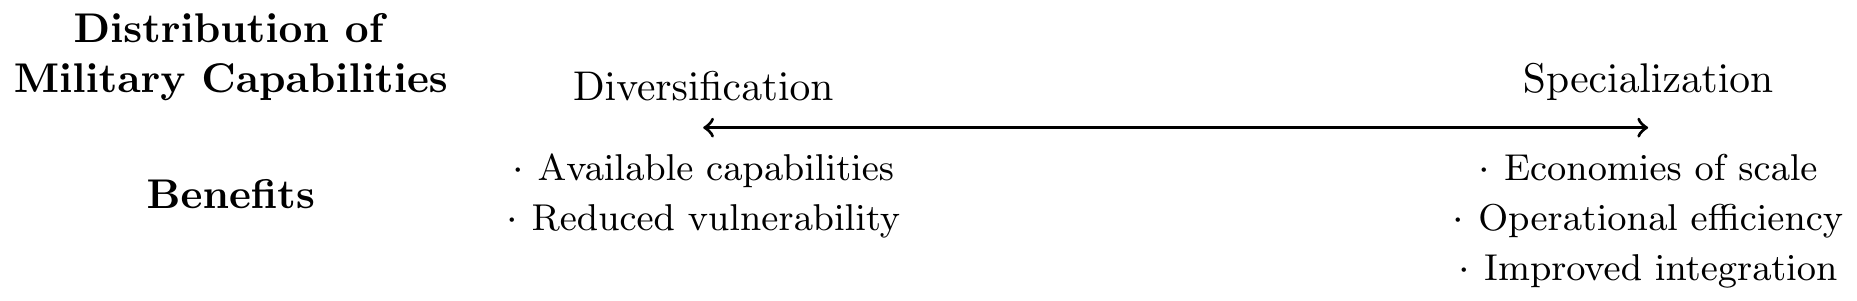
\includegraphics{2023-04-04_Specialization_files/figure-pdf/fig-spectrum_specialization-1.png}

}

\caption{\label{fig-spectrum_specialization}Varieties of a state's
distribution of military capabilities.}

\end{figure}

First, the cost of setting up manufacturing and acquiring the materials
for weapons acquisition entail large upfront investment. But the
marginal cost of that investment goes down as a state decides to produce
more of the same asset (Markowski and Hall 1998). For example, Germany
has reduced the need for redundant infrastructure by centralizing car
and light truck production all within the Bundeswehr-Fuhrparkservice
GmbH which allows them to produce newer but less varied vehicles more
quickly (Overhage 2013). Economies of scales are also ``active'' in that
they accrue as a state undertakes defense-related activities, so the
more a state operates with a particular asset, the lower their marginal
costs because of ``learning by doing'' (Postrel 2002). Even states that
are primarily ``arms buyers'' as opposed to ``arms builders'' experience
reduced maintenance and repair costs from a shorter list of components
and end-use products.

Second, specialization allows a military to perform select missions more
efficiently by streamlining logistics and reducing the overall cost of
learning how to use new equipment. Many assets require
capability-specific investments that involve a fixed cost. A state with
several dozen different types of aircraft will require more complex
pilot training than a state that only has to master the effective use of
a few types of aircraft. One source of NATO's debate over who should
send main battle tanks to Ukraine concerns Ukraine's familiarity with
how those more complex systems work; they could immediately operate T-72
tanks sent from Eastern Europe, but training and logistics for the US
Abrams tank would take months (Lanoszka and Becker 2023, 6--10).

Third, integration is easier as a country specializes since the
complexity of integrating numerous types of platforms with various roles
and responsibilities decreases. Even issues as fine-grained as the
software used in various pieces of equipment are sufficient impediments
to military operations that nations consider this issue carefully.
NATO's Standardization Agreement (STANAG), for example, ensure broad
fleet compatibility with the same fuel nozzle. In 2019, Jordan gave up
its Chinese-built CH-4 drone fleet because successful integration with
other platforms was going to require a costly overhaul of their entire
communications system (Penney 2020).

In contrast to specialization, the benefits of diversification concern
the security gains of a full-spectrum military that makes combined arms
warfare possible (Biddle 2005). States that engage in a full-spectrum
approach to warfare instead of specializing benefit from having more of
the capabilities needed to defend themselves. No weapons system is
perfect, and the nature of warfare means weapons systems that excel at
one aspect of international conflict do so precisely because they lack
other abilities. Aerial bombers sacrifice maneuverability so that they
have carry a high payload. But more maneuverable aircraft like fighters
achieve the benefits of speed with lower ordinate payloads. Far from
just a tactical consideration, this diversification is a political and
strategic concern since higher-order state objectives like credibility,
effectiveness, and efficiency are advanced by military platforms in
varying and often zero-sum ways. ``Military specialization imposes
opportunity costs in terms of what a nation does well and where it must
compromise its capabilities. Choices about what to buy, and where and
how to field the nation's military might, then pose certain constraints
on political strategy'' (J. R. Lindsay and Gartzke 2022, 346).

Diversification also reduces vulnerability by making it more difficult
for the adversary to develop countermeasures. A state with a limited
variety of assets has given their adversary a shorter list of
capabilities they must be able to defeat to prevail in combat. Air
defense systems, for example, come in three different varieties;
surface-to-air missiles (SAM), anti-aircraft artillery (AAA), and
aircraft armed with air-to-air missiles (AAM). These systems all differ
in the altitudes they can target, stealth, reaction times, mobility, and
cost. In a 1940 testimony before the Senate Appropriations Committee,
General George Marshall noted the need for both aircraft and
anti-aircraft artillery because the former is an area system that excels
at searching while the latter is a point system designed to protect key
assets. When asked by Congress which was most important he said all of
them; ``the whole thing is interwoven\ldots all these matters have to be
given proper weight to get a well integrated and balanced whole''
(Hammel 2010). A state that has chosen to develop only one of these
capabilities might have more in quantity (scale economies) and quality
(operational efficiency and improved integration), but they are now
vulnerable to the development of new missiles and aircraft designed to
circumvent the strengths of their adversary's one air defense system
(Gartzke, Kaplow, and Mehta 2014, 484--85).

Former US Chairman of the Joint Chiefs of Staff Colin Powell (2010, 157)
described a diverse, full-spectrum force as involving the ability to
``prevail, quickly, and cheaply, in any and all forms of conflict''.
States that have not embraced this model have consequently suffered.
After the Yom Kippur war, Israel opted to specialize their military by
cutting artillery and mechanized infantry in favor of a shift to pure
armor-aircraft. This left them vulnerable to an anti-armor and
anti-aircraft attack that set them back in the early stages of the 1973
Arab-Israeli War. It was only after they reversed course that they were
able to defeat the Egyptian air defense systems (Herzog 2018). After
World War II, India's Naval Plan Paper (1947) made the case for a
``balanced naval task force'' which was later explained by Vice Admiral
Parry (1949) as a move to reduce India's vulnerability with a navy
``containing all types of ships and aircrafts, on the sea, over the sea,
and under the sea''.

\hypertarget{allies-increase-specializations-payoff}{%
\subsection{Allies Increase Specialization's
Payoff}\label{allies-increase-specializations-payoff}}

Even well-resourced states experience difficulty excelling at all forms
of conflict simultaneously (D. R. Lake 2012, 91). Making priorities is
both a product of luxury and of necessity. An actor can overcome this
constrained optimization problem and minimize the trade-off between
efficiency and efficacy through security cooperation.\footnote{This
  theory is derived from business organization research on inter-firm
  cooperation (Gulati, Nohria, and Zaheer 2000; Meier, Stephenson, and
  Perkowski 2019).} Working with partners allows for individual
functional specialization under the auspices of a broader defense
arrangement. A parsimonious way to think about this in the international
context is defense alliances, since they are an indication of the two
prerequisites for security cooperation with a committed partner: (1)
belief in a partner's willingness to play a role in improving your
well-being and (2) their ability to do so (Morrow 1994; Leeds
2003).\footnote{These two conditions exist more generally for
  theoretical cooperation (Deutsch 1962). I choose the language
  ``well-being'' rather than ``security'' because this also applies to
  asymmetric alliances where instead of seeking protection, the dominant
  state may be seeking autonomy to advance pursuit of its preferred
  foreign policy outcomes (Morrow 1991, 907--9).} Specialization is thus
not a questionable prioritization of efficiency by states choosing to
forgo the security benefits of a diversified military, but instead a way
to get the best of both worlds made possible by architectures of
international cooperation.

Alliances increase the payoffs of military specialization in a few ways.
Having allies who you believe will come to your defense allows a state
to allocate resources toward non-security functions since defense
resources are aggregated. In spending less on your own militarily, you
can under-invest in certain capabilities that have high marginal
production cost at current levels. Practitioners have recognized how the
resource re-allocation benefits of alliances translate to focused
specialization. US Naval Rear Admiral M. E. Smith (2013) noted that by
having a cooperative approach, ``each nation can avoid duplication and
thereby reduce its proportional share of the expense. This
is\ldots about a focused and pragmatic approach to force allocation that
acknowledges allies' existing contributions. Countries could immediately
apply the freed resources to unique national missions.''

Second, the resource gains under cooperation are more than the sum of
their parts because of scale economies. Collective defense can be more
than the sum of its parts if specialized actor bring a smaller variety
of capabilities to the table, but more of them. Discussions in the US
about a `1,000 ship Navy' are predicated on precisely this model; ``a
voluntarily global maritime network that ties together the collective
capabilities of free nations to establish and maintain a dramatically
increased level of international security in the maritime domain''
(Morgan and Martoglio 2005). Similarly, the 2002 Prague Summit outlined
8 areas over which NATO states could try to specialize, which 2011
Chicago Summit advocated as ``certain countries should let go of certain
capabilities in order to create a more rational defence structure from a
Brussels perspective'' (Christiansson 2013, 181--86).\footnote{Auerswald
  and Saideman (2014, 229--33) also point out specialization can help
  individual states engage in cost-effective defense investments while
  maintaining an aggregate full-spectrum allied force, but are skeptical
  trust issues can be overcome.} This resulted in Czechia specializing
in CBRN defense, Denmark omitting submarines, the Baltic states
emphasizing cyber defense at the expense of fighter aircraft, and a
handful of states taking the lead on strategic airlift.

Alliances that vary in their structure and purpose will also vary in the
mechanism by which they incentivize specialization (Leeds, Mattes, and
Vogel 2009; Mattes 2012). Specialization may be the product of high
interest alignment resolving coordination problems or hierarchy reducing
the risk of opportunism coercively or contractually (Gannon 2021a). But
theorizing the conditions under which some alliances are more or less
likely to induce specialization risks putting the cart before the horse
without initial evidence that alliances influence the composition of a
state's arms portfolio at all. Linking alliance membership with higher
military specialization is a necessary precursor, setting the foundation
for differentiating alliances based on the mechanisms by which
specialization occurs and which alliance members specialize in what.

In sum, force structures that omit useful defense capabilities and/or
overproduce others can occur when a state has opted to specialize its
military portfolio. A state is more willing to do so when the security
risks of specialization are no longer prohibitive; a condition made
possible by alliance relationships that resolve the constrained
optimization problem. Shared defense thus garners the security benefits
of capability aggregation posited by the neo-realists (Parent and Rosato
2015) as well as the economic benefits put forth by hierarchy theorists
(D. A. Lake 2001, 147--51).

\hypertarget{sec-empirics}{%
\section{Empirical Analysis}\label{sec-empirics}}

\hypertarget{dependent-variable}{%
\subsection{Dependent Variable}\label{dependent-variable}}

The dependent variable is the degree of specialization of a state's
distribution of military capabilities in a given year. A state's
distribution of military capabilities is defined here as the combination
of military equipment that could be used by a state during conflict.
This includes platforms like artillery, aircraft, naval vessels, armored
vehicles, satellites, and transport ships.\footnote{The data do not
  include munitions like single-use bombs or ammunition or firearms used
  by individual military personnel. Existing research has made similar
  distinctions in what military capabilities are examined
  cross-nationally (Brooks and Wohlforth 2016).} I choose these scope
conditions because military platforms are equipment that can be
deployed, that other nations are likely to observe, that could be used
to signal intent and resolve in a crisis without actual use, and that
are durable goods.\footnote{While platforms and capabilities are not
  synonymous, there are here categorized based on their role/mission
  which serves as a reasonable proxy for capabilities. For example,
  fighter aircraft differ from bomber aircraft in what they allow a
  state to do, and those differ yet still from transport or tanker
  aircraft.} The index is constructed using the rDMC dataset detailing
annual counts of 69 different military platforms across all states from
1970-2014 (Gannon 2021b).

To measure military specialization at the country-year level, I create
an index quantifying the differences across states' distribution of
military capabilities identified as omissions and over-productions
relative to the neorealist baseline assumption that states behave as
like-units under anarchy and should consequently seek similarly diverse
military capabilities subject to resource constraints. Assume that
global defense in year \(t\) is composed of \(N\) countries and \(M\)
military technologies. I construct an \(n \times m\) interaction matrix
for each year \(t\) such that each row \(n\) is a country and each
column \(m\) is a technology. Each cell thus represents the observed
count of a given technology in that country-year's military. In
aggregate, this can be represented as
\(d_j = \sum_{i=1}^{N}(p'_{ij}ln\frac{p'_{ij}}{q_i})\) where \(N\) is
the total number of countries in that year, \(p_{ij}\) is country
\(i\)'s possession of technology \(j\) divided by the total amount of
technologies \(j\), and \(q_i\) is the total number of technologies
possessed by country \(i\) divided by the total number of technologies
in the world.\footnote{This bipartite network structure is modeled after
  its use in ecological research (Alarcón, Waser, and Ollerton 2008).}

From this, I calculate the functional entropy of each country's military
using a trait-based similarity measure drawn from Rao's (1982) quadratic
entropy calculation of the average difference across technology
portfolios between each country and all other countries in a given year
weighting the technologies by their relative abundance. This calculates
the functional entropy of a country's military as:
\(R(p_i,D) = \sum_{k=1}^{S} \sum_{l=1}^{S} \sqrt{(p_k|i)} \sqrt{(p_k|j)} d_{kl}\)
where \(p_i=(p_1|i, …, p_k|i, …, p_S|i)\) is the vector of relative
technology abundance within country \(i\); \(S\) is the number of
technologies; \(D=(d_kl)\) is the matrix of functional dissimilarity
between the technologies, and \(d_kl\) is the functional dissimilarity
between countries \(k\) and \(l\) (Pavoine 2020).\footnote{As this
  measure of functional entropy is developed by Pavoine et al. (2017),
  its formula is provided verbatim. In the original statistical ecology
  application, this measure uses Hill (1973) numbers to measure the
  dissimilarity between biological species based on observed traits,
  accounting for the rarity of those traits.}

To provide some intuition, this measure of entropy calculates the degree
of surprise or unpredictability produced by the difference between the
amount of a military capability we expect a country to possess and what
that country actually possess. This prior expectation is based on the
distribution of technologies across all other states and within the
state in question, thus providing a relative and absolute measure. For
example, if most states possess, on average, twice as many transport
helicopters as they do transport aircraft, we would expect a state with
10 transport aircraft to have roughly 20 transport helicopters. But if
the state in question already possessed many more transport aircraft
than everyone else, we would update our expectation since we know a way
this quantity differs from other states and other capabilities. Our
expectation for transport helicopters can thus be \emph{re}-calibrated
based on (1) the number of transport aircraft this states possesses
relative to everyone else's transport aircraft, and (2) the number of
transport aircraft this state possesses relative its other capabilities.
If we now reproduce this method across all other capabilities, we get a
revised prior expectation for the capability in question - transport
helicopters. The closer the observed quantity is to our final
re-calibrated expectation, the less entropy the quantity produces, and
thus the lower the level of specialization since producing many more or
far fewer transport helicopters than the model expects are both
indications that the state has absolute and relative specialization by
omitting or over-producing that capability relative to intra-state and
interstate expectation.

Figure~\ref{fig-spec_scores} shows the distribution of this index across
all observations.\footnote{There is a small, statistically significant,
  positive temporal trend in specialization that is accounted for in the
  statistical model. Technology evolves dynamically, in this case maybe
  due to shifts away from high-quantity legacy systems towards
  high-quality expeditionary warfare systems (Terriff, Osinga, and
  Farrell 2010; Schnaubelt 2011).} Among the most specialized
observations are Japan after 2010 and the least specialized include the
Baltic states in the early 1990's. Given the number of destroyers and
offshore coastal ships Japan possesses, having almost no amphibious
ships is an unexpected form of naval specialization (in the entropic
sense). So while Japan may dominate in many military capabilities, that
does not mean its relative dominance is equal across the board. Even the
United States has specialized, with famous underproductions including
the lack of minesweepers during the 1984 Iran-Iraq Tanker War (DeVore
2009), nuclear, chemical, and biological (NBC) reconnaissance vehicles
at the start of the 2003 Iraq War (Geis 2013, 241--55), and icebreakers
in recent years (Markowitz 2020). Importantly, having a diversified
military is not synonymous with having a lot of everything. States can
have very little of everything, making them similarly \emph{in}capable
across the board.\footnote{Almost all states possess certain
  capabilities like light transport aircraft and search and rescue
  helicopters. This is consistent with accounts of basic infrastructure
  ensured by ``critical assets'' (Matláry and Østerud 2007) and
  identifies the importance of accounting for economic capacity to
  ensure the specialization index is not simply measuring the luxury of
  economic choice.}

\begin{figure}[h]

{\centering 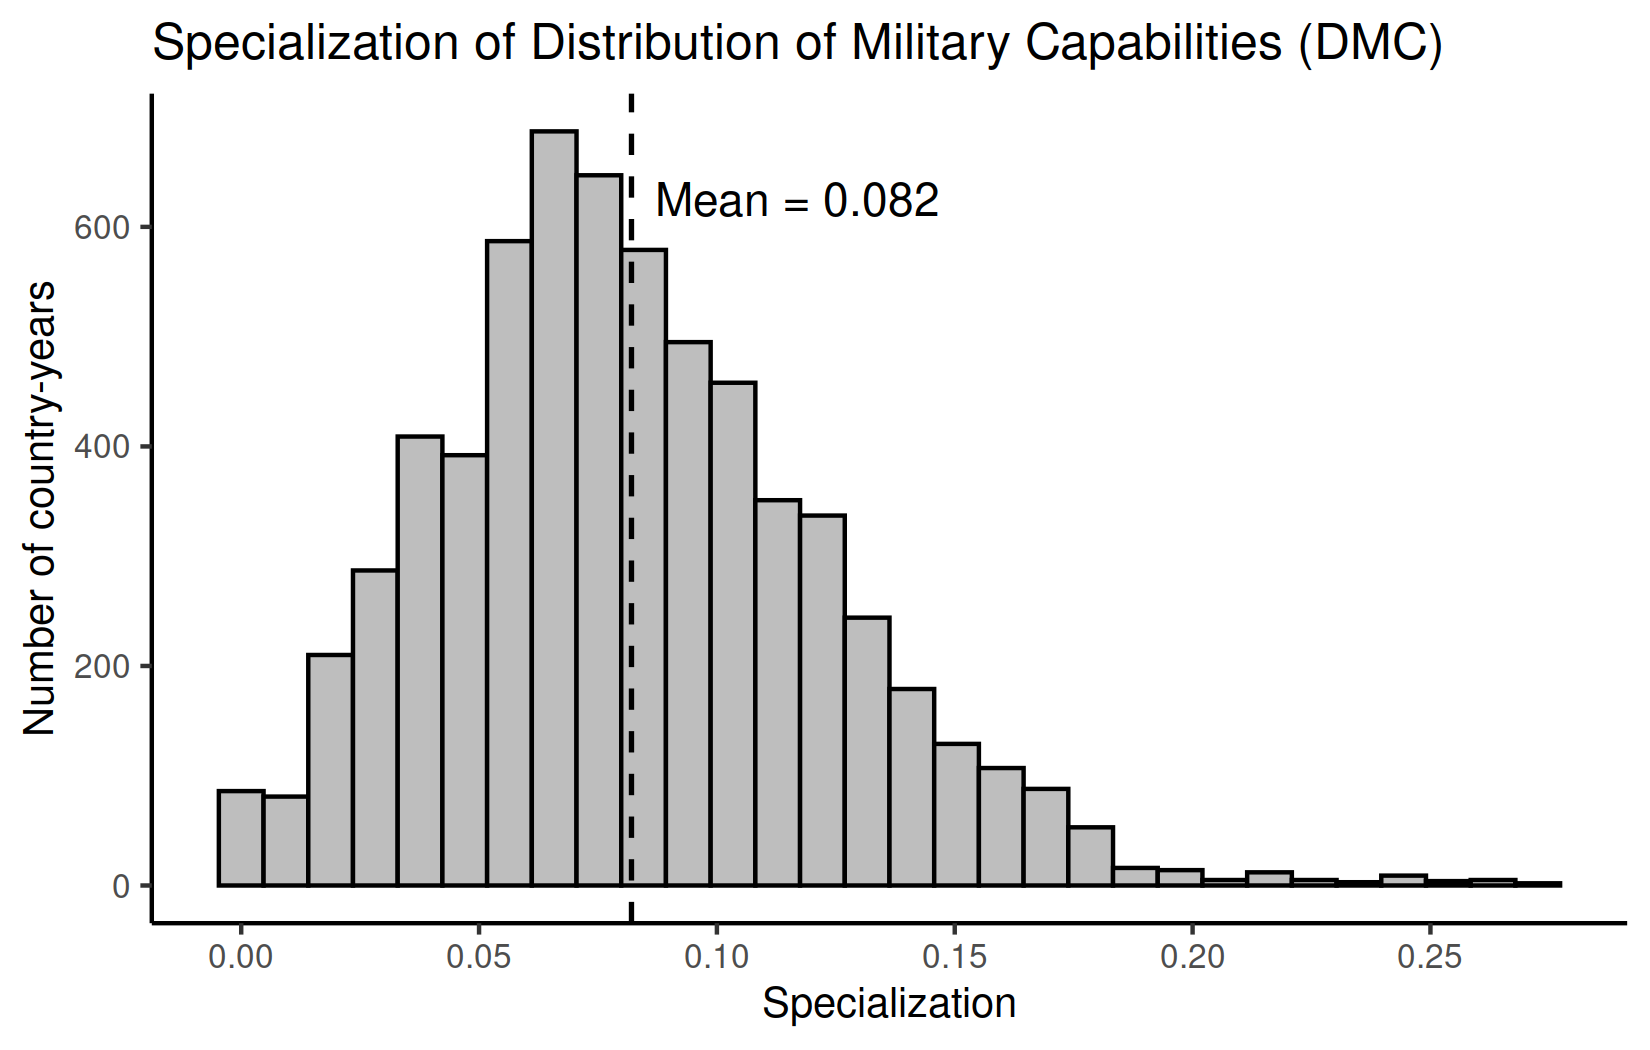
\includegraphics{2023-04-04_Specialization_files/figure-pdf/fig-spec_scores-1.png}

}

\caption{\label{fig-spec_scores}Distribution of country-year military
specialization. The measure is bounded between 0 and 1, with 1
representing the highest theoretically possible level of
specialization.}

\end{figure}

\hypertarget{independent-variable-and-controls}{%
\subsection{Independent Variable and
Controls}\label{independent-variable-and-controls}}

The independent variable measures a state's alliance
relationships.\footnote{Data on state participation in defensive
  alliance pacts is provided by the Alliance Treaty and Provisions
  (ATOP) dataset, version 5 (Leeds et al. 2002).} A state's allies are
those with whom it has a defensive alliance pact whereby the partner
state has made a promise to defend the state in question. As most states
have at least one formal treaty ally in a given year, existing research
using alliances as an independent variable has proxied for the
importance of a state's allies to that state's security. I
operationalize alliances at the country level two different ways; (1) as
the logged sum of military spending of a state's allies (excluding
itself) (DiGiuseppe and Poast 2016) and (2) the ratio between a state's
CINC score and the sum of their alliance CINC scores (including itself)
(Fang, Johnson, and Leeds 2014; Johnson, Leeds, and Wu 2015). For both
variables, higher values indicate more militarily-capable alliance
relationships which serves as an observable indicator of conditions
conducive to military specialization. Because a formal defense
commitment suggests a mutual belief in a partner's willingness and
ability to provide defense, a state with more militarily-capable allies
should be more confident that specializing its military will not leave
it vulnerable (A. Smith 1995; Benson and Clinton 2016).

I include a set of control variables that existing theories indicate
could be causally related to the dependent and/or independent variables
of interest. The models control for regime type, coding a country as a
democracy if they score higher than 6 on the 21-point Polity V index.
Democracies may spend less on defense (Fordham and Walker 2005), build
more capital-intensive militaries (Gartzke 2001), and be more
(DiGiuseppe and Poast 2016) or less (Gartzke and Gleditsch 2004)
reliable partners. There is also a control for whether a country has
been involved in an interstate war in the previous half decade, as a
salient threat environment (Ghosn, Palmer, and Bremer 2004) or recent
conflict experience may change patterns of innovation (Kollars 2015).
The models control for GDP, as resource-constrained states may be unable
to invest in a diverse array of military capital (Diehl 1994) or may
shift defense funds from platforms to personnel due to unemployment
(Becker 2021).\footnote{``Tech-flation'' could explain why higher
  security costs cause militaries to adopt fewer, but higher performing
  platforms (Adelman and Augustine 1990), although the empirical record
  in Europea suggests states diversify their military portfolios despite
  the financial cost of doing so (Howorth 2007).} Finally, I control for
CINC scores, as states harboring global ambitions may invest more in
power projection capabilities (Markowitz and Fariss 2018).\footnote{In
  addition to having unclear expectations about their relationship to
  specialization, time-invariant geographic variables are addressed via
  fixed effects models in the appendix rather than constant model
  parameters that risk model degeneration (Beck 2011).}

\hypertarget{model-and-results}{%
\subsection{Model and Results}\label{model-and-results}}

The dependent variable is military specialization of country \(i\) in
year \(j\), measured with the functional entropy index described above.
Higher values indicate more specialization and less diversification. As
the dependent variable is continuous, I estimate a series of ordinary
least square (OLS) regressions using the two different independent
variables - (1) logged sum of allied military spending, (2) ratio of a
country's CINC score to that of all its allies and itself. For each
independent variable, I estimate a bivariate model country-clustered
standard errors to account for the non-independence between observations
in panel data (Cameron and Miller 2015) then a model that adds all
control variables and year scaled cubic polynomials to account for
temporal specialization trends (D. B. Carter and Signorino 2010).

Table~\ref{tbl-results} shows the results of all four models. Models 1
and 2 demonstrate allied military spending is positively associated with
military specialization with statistical significance of at least the
0.05 standardized level. Although allies' CINC ratio is negative
associated with military specialization in the bivariate model (Model
3), the inclusion of control variables and temporal dependencies (Model
4) reverses the association, which is consistent with the other models
and theoretical expectations. In aggregate, these results provides
suggestive evidence that states that have militarily-capable alliance
partners have more specialized military portfolios - omitting certain
capabilities and over-producing other capabilities - relative to states
that are reliant upon self-defense.

I present the OLS results here as they are most easily interpretable and
consistent with modeling specifications in existing research with
similar data. Nonetheless, these results are robust to a series of
alternate model specifications provided in the appendix that relax
assumptions about the underlying distribution of the dependent variable
and temporal and country-specific trends. Similar results are found
using fractional logit and beta regressions, Bayesian zero-inflated and
ordered beta regressions, and with alternate fixed effects and standard
error clustering specifications.

\hypertarget{tbl-results}{}
\begin{table}
\caption{\label{tbl-results}Military Specialization and Alliances, Multivariate Analysis }\tabularnewline

\centering
\begin{tabular}[t]{lcccc}
\toprule
  & (1) & (2) & (3) & (4)\\
\midrule
Allies' Mil Spend. (log) & \num{0.004}*** & \num{0.001}* &  & \\
 & (\num{<0.001}) & (\num{0.035}) &  & \\
Allies' CINC Ratio &  &  & \num{-0.045}* & \num{0.025}*\\
 &  &  & (\num{0.022}) & (\num{0.035})\\
Democracy &  & \num{-0.002} &  & \num{0.000}\\
 &  & (\num{0.515}) &  & (\num{0.958})\\
Interstate War (5yr lag) &  & \num{0.001} &  & \num{0.002}\\
 &  & (\num{0.846}) &  & (\num{0.674})\\
GDP (log) &  & \num{0.012}*** &  & \num{0.013}***\\
 &  & (\num{<0.001}) &  & \vphantom{3} (\num{<0.001})\\
CINC &  & \num{0.183} &  & \num{0.203}\\
 &  & (\num{0.293}) &  & (\num{0.278})\\
Year &  & \num{0.006}*** &  & \num{0.006}***\\
 &  & (\num{<0.001}) &  & \vphantom{2} (\num{<0.001})\\
Year$^2$ &  & \num{0.000}*** &  & \num{0.000}***\\
 &  & (\num{<0.001}) &  & \vphantom{1} (\num{<0.001})\\
Year$^3$ &  & \num{0.000}*** &  & \num{0.000}***\\
 &  & (\num{<0.001}) &  & (\num{<0.001})\\
\midrule
Num.Obs. & \num{4629} & \num{3900} & \num{4568} & \num{3900}\\
AIC & \num{-7400.7} & \num{-9085.7} & \num{-7079.8} & \num{-9067.4}\\
BIC & \num{22397.6} & \num{15306.0} & \num{22265.1} & \num{15324.2}\\
\bottomrule
\multicolumn{5}{l}{\rule{0pt}{1em}+ p $<$ 0.1, * p $<$ 0.05, ** p $<$ 0.01, *** p $<$ 0.001}\\
\multicolumn{5}{l}{\textsuperscript{a} All models include country-clustered standard errors.}\\
\end{tabular}
\end{table}

The relationship between alliances and military specialization is also
substantively significant. Holding all control variables constant, a one
standard deviation increase in allies' CINC ratio (independent variable
in Models 3 and 4) is associated with a 1.4\% increase in a state's
military specialization; the difference in Japan's military
specialization between 1982 and 2000. Despite what what is traditionally
understood as a lopsided division of security responsibilities, the US
and Japan have each specialized their security responsibilities
intentionally (Ando 2015). Japan's 1982 capability realignment described
in Section~\ref{sec-intro} signaled the start of a new era of
cooperation with the United States, with the joint communique issued by
Prime Minister Suzuki and President Reagan (1981, 3) stressing ``the
desirability of an appropriate division of roles between Japan and the
United States''. Japan was entrusted with protecting its sea lines of
communication (SLOCs) 1,000 nautical miles off its coast and providing
logistical support to offensive US operations as needed.
Figure~\ref{fig-japan} illustrates how one result of this strengthened
alliance was a more specialized Japanese military. Japan doubled its SAM
and far-from-shore naval capabilities like destroyers and utility
helicopters and significantly downsized its amphibious and coastal
fleets. The alliance relationship with the United States allowed Japan
to carry the ``defensive shield'' by specializing in capabilities for
SLOCs and rear-area support while forgoing ``offensive spear''
attack-capable surface ships and high-tech long-range aircraft (Schoff
2014).\footnote{This case illustrates an important avenue for future
  research - the degree to which specialization at the dyad or
  alliance-level is complementary. An allies' defense portfolio can
  compensate for a given state's specialization by possessing the
  capabilities the given state is missing or by possessing a diversified
  full-spectrum force. The former suggests the reliance is
  unidirectional, while the latter suggests a degree of mutual
  interdependence.}

\begin{figure}[H]

{\centering 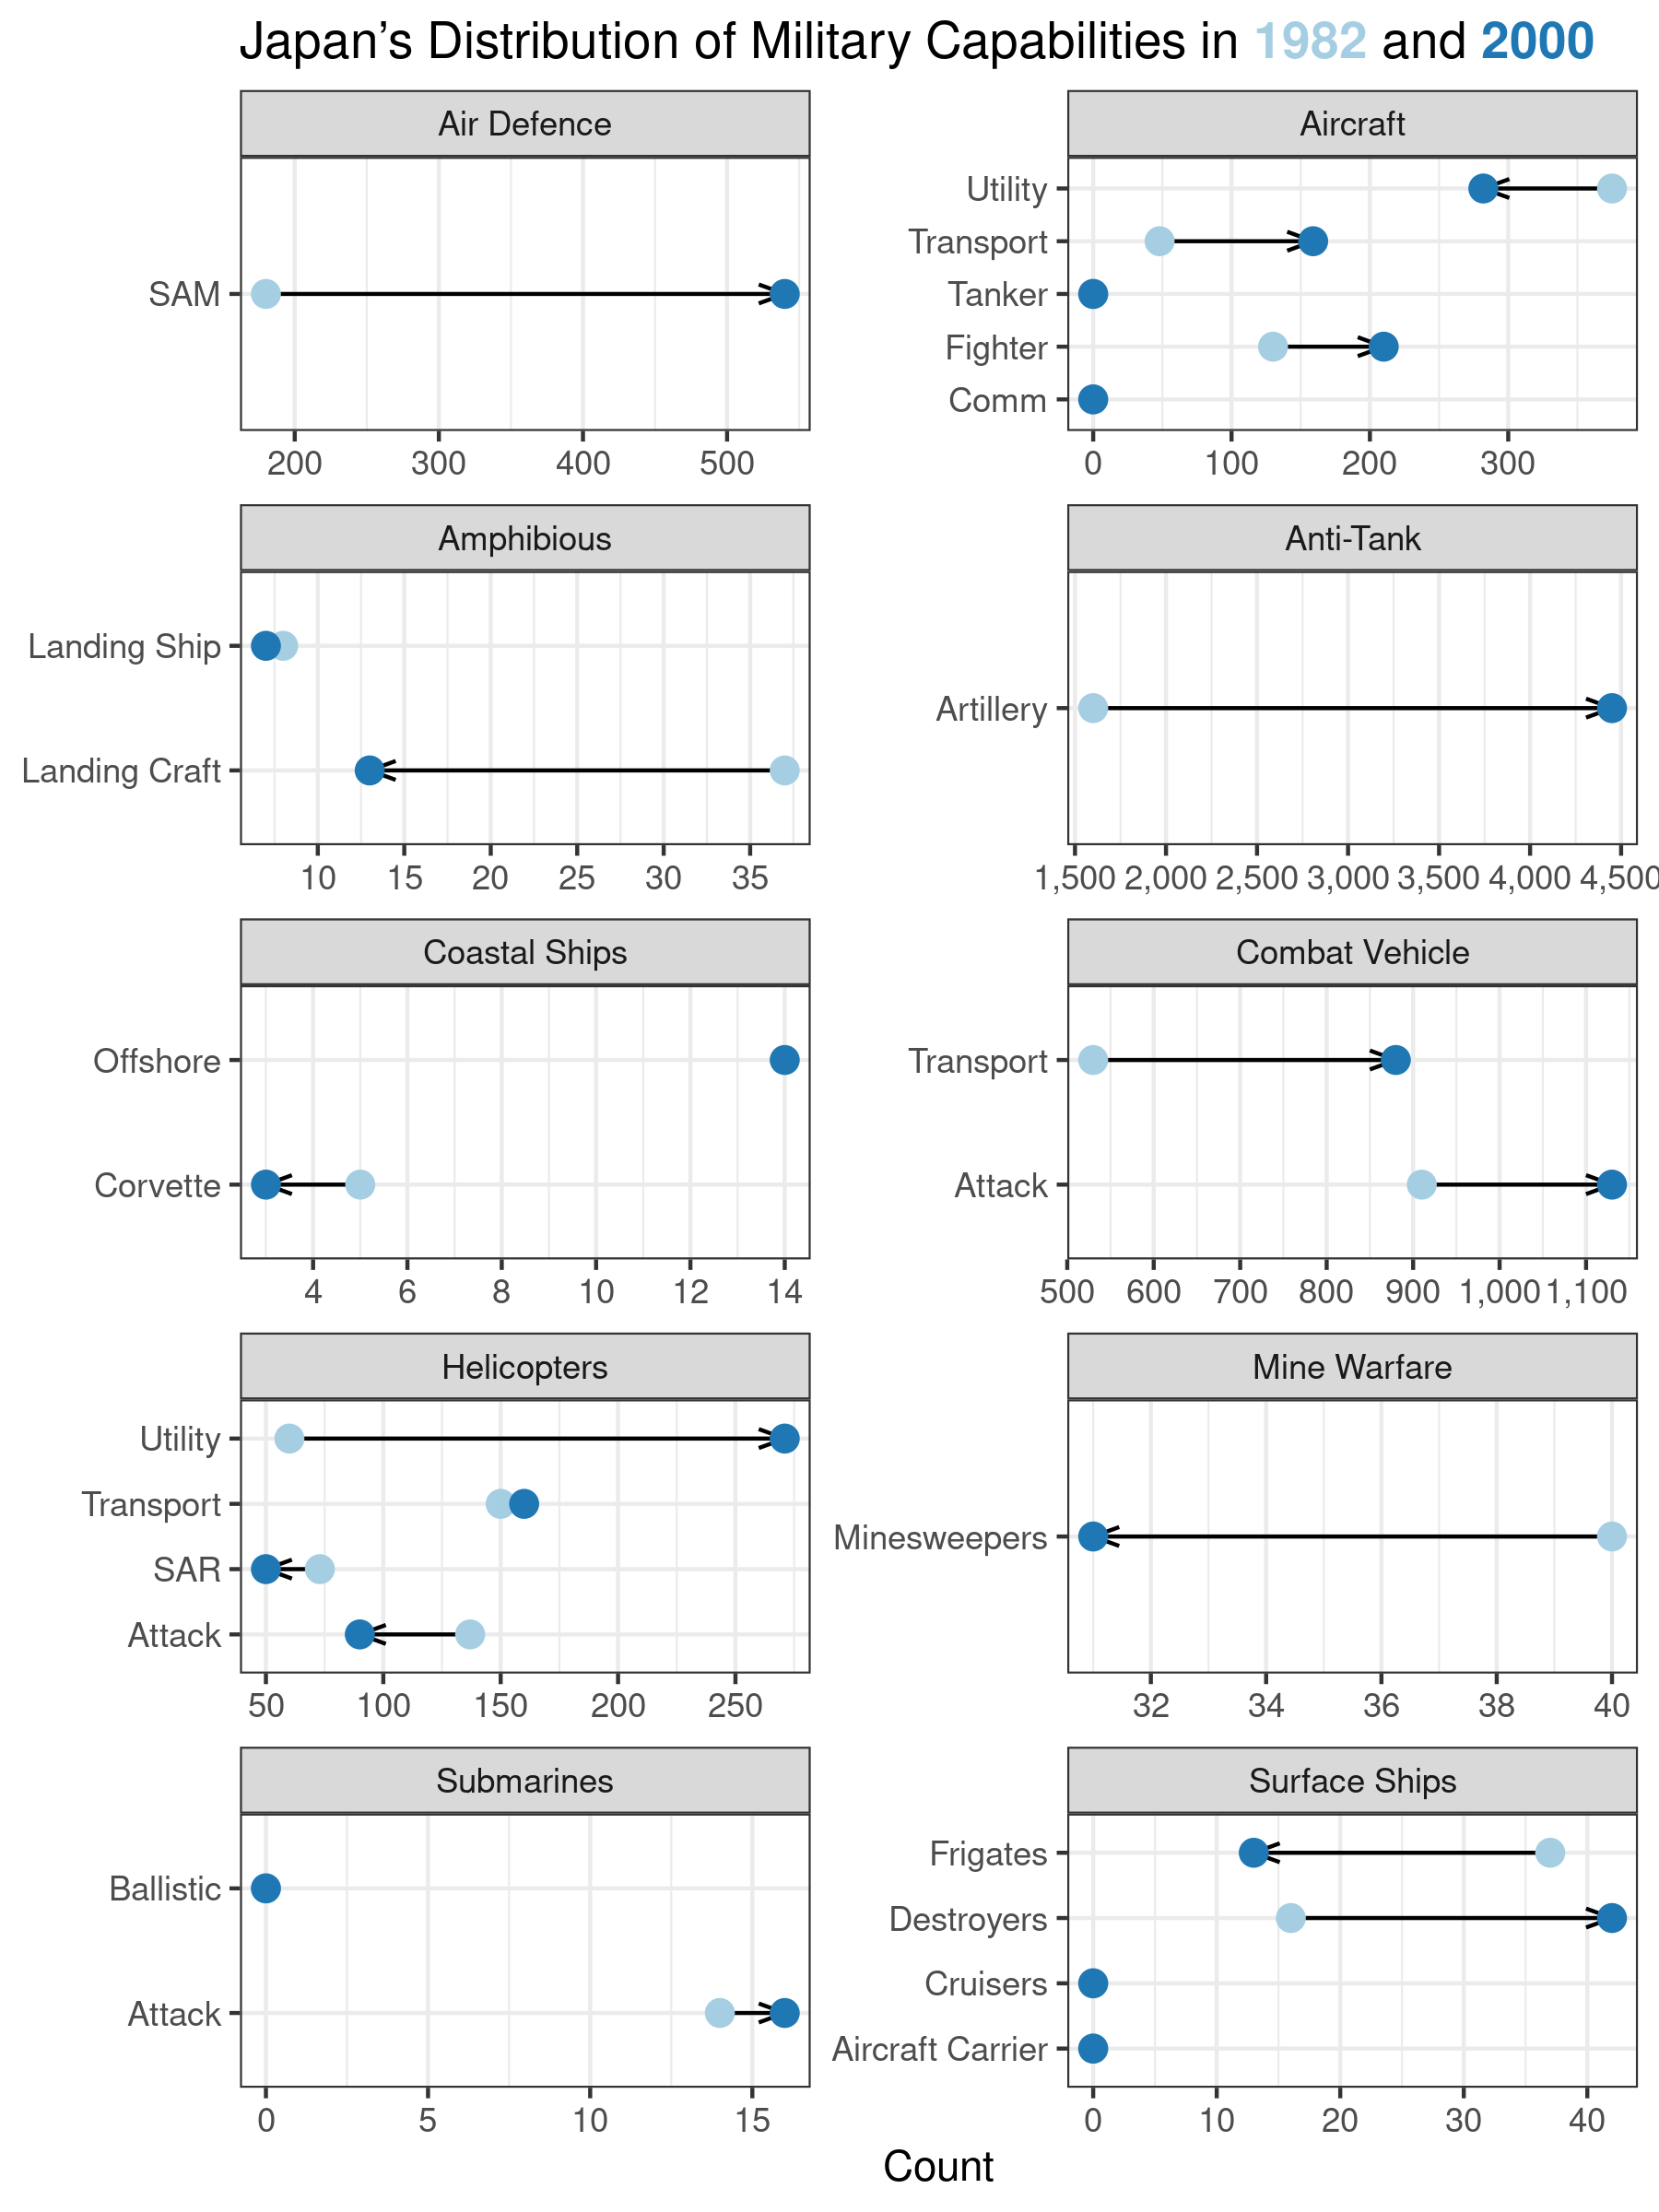
\includegraphics{2023-04-04_Specialization_files/figure-pdf/fig-japan-1.png}

}

\caption{\label{fig-japan}Change in Japan's distribution of military
capabilities between 1982 and 2000. Capabilities Japan did not possess
at any point during this time period (eg ballistic missiles and drones)
are omitted.}

\end{figure}

\hypertarget{sec-conclusion}{%
\section{Conclusion}\label{sec-conclusion}}

Despite recognition that how states spend their defense dollars matters
(Kunertova 2017; Becker et al. 2022), research has largely failed to
identify ways military portfolios vary, nonetheless explain that
variation. This paper focuses on one important dimension on which
military portfolios vary - their degree of specialization - and the role
that alliances play in explaining that variation. The conventional
understanding about a state's choice to provide for their security
internally (arms) or externally (allies) requires understanding that
alliance relationships influence not just the amount, but also the
\emph{composition} of a state's armaments. This intersects importantly
with the guns versus butter trade-off because of the economic
implications of the decision to have a military composed of a few
specialized assets or a broadly diversified force.

Debates about the value of alliances often turn to the costs of alliance
commitments (Alley and Fuhrmann 2021; Cooley et al. 2022) and
burden-sharing (Blankenship 2021; Becker et al. 2023). Security
cooperation allows states to ``take advantage of economies of scale in
the provision of defense and to benefit from specialization by
coordinating training, equipment, and procedures. By pooling their
efforts and/or cooperating with states that have different comparative
advantages, leaders hope to create a stronger joint fighting force''
(Leeds and Anac 2005, 185). By advancing discussion from burden-sharing
\emph{costs} to burden-sharing \emph{configurations}, new perspectives
on the value of alliances emerge (Gannon 2022).

Then US ambassador to NATO Ivo Daalder (2013) noted that the problem was
not that NATO countries were not spending enough on defense, it was that
they were not spending that money wisely. This paper substantiates
specialization as a novel mechanism by which alliances can reduce
states' military spending by providing ``greater security with fewer
resources but more coordination'' (Rasmussen 2011). As economic
pressures maximize the importance of avoiding wasteful defense spending,
allies can turn to specialization to ensure that spending is efficient
while still being efficacious. As UK Secretary of Defence Hammond (2012)
explained, the answer to this economic pressure lies in ``prioritizing
ruthlessly, specializing aggressively, and collaborating
unsentimentally.''

But specializing one's military because of reliance on others is not
without its risks, as there is always a ``fear that the other will not
live up to the terms of the agreement'' (D. A. Lake 1996, 15). Japan and
South Korea's defense strategies have remained neither static nor the
same. Contemporary discussions about militarization in response to
Chinese, North Korean, and Russian threat have put their respective
alliances with the US front and center. To the degree that Japan has
specialized their military in forgoing and/or overemphasized certain
capabilities because of their relationship with the United States, their
ability to defend themselves in the event of attack may be compromised.
South Korea may be trending in the opposite direction, signaling their
discontent with the alliance by publicly contemplating the need to
duplicate uncertain US nuclear protection with an arsenal of their own
(Lind and Press 2023). More generally, if states feel confident they can
rely on their allies, we should see them continue to specialize their
militaries. Conversely, allies beginning to diversifying their military
portfolios may be hedging their bets in seeking to defend themselves
with a full-spectrum force rather than risk the consequences of
abandonment.

Future inquiries should explore several critical avenues. Defense
cooperation takes many governance forms that allow states to rely on
each other to different degrees and for different reasons (Benson 2012).
The analysis here simply looks at defense pacts using existing
operationalizations of reliability. But differences across alliances in
joint war planning (Poast 2019a, 174--75), the threat environment (Niou
and Zeigler 2019), and domination (Lanoszka 2013) may influence who
specializes in what and the degree to which specialization by partners
produces a coordinated and complementary division of labor. Future work
could also look at the size of alliances (Fordham and Poast 2016),
specialization across issue areas like diplomacy or economics (Kinne and
Bunte 2020), or different security alignments like defense cooperation
agreements (DCAs) (Kinne 2020) and ad-hoc coalitions (Kreps 2011;
Cappella Zielinski and Poast 2021).

Even if states' fear of exploitation is most salient where survival may
be at stake, specialization is evidence states can manage uncertainty
about cooperation under anarchy by increasing its expected benefits.
This does not necessarily run counter to conventional wisdom about
military portfolio diversification, but it does question the common
belief that internal balancing and imitation - even in the face of a
common enemy - is the best form of defense in the self-help world of
anarchy. One of the reasons alliances are created in the first place is
to change states' defense spending and their military portfolio. Rather
than think about arms and allies are distinct strategies for security,
we should recognize that the arms a state develops are a function of the
arms of its allies.

\newpage

\hypertarget{references}{%
\section*{References}\label{references}}
\addcontentsline{toc}{section}{References}

\hypertarget{refs}{}
\begin{CSLReferences}{1}{0}
\leavevmode\vadjust pre{\hypertarget{ref-adelman_defenserevolutionstrategy_1990}{}}%
Adelman, Kenneth L., and Norman R. Augustine. 1990. \emph{The Defense
Revolution: Strategy for the Brave New World}. {San Francisco, Calif. :
Lanham, Md}: {ICS Press}.

\leavevmode\vadjust pre{\hypertarget{ref-alarcon_yeartoyearvariationtopology_2008}{}}%
Alarcón, Ruben, Nickolas M. Waser, and Jeff Ollerton. 2008.
{``Year-to-Year Variation in the Topology of a
Plant\textendash pollinator Interaction Network.''} \emph{Oikos} 117
(12): 1796--1807.
\url{https://doi.org/10.1111/j.0030-1299.2008.16987.x}.

\leavevmode\vadjust pre{\hypertarget{ref-alley_budgetbreakerfinancial_2021}{}}%
Alley, Joshua, and Matthew Fuhrmann. 2021. {``Budget {Breaker}? {The
Financial Cost} of {US Military Alliances}.''} \emph{Security Studies}
30 (5): 661--90. \url{https://doi.org/10.1080/09636412.2021.2021280}.

\leavevmode\vadjust pre{\hypertarget{ref-allison_armamentsarmscontrol_1975}{}}%
Allison, Graham T., and Frederic A. Morris. 1975. {``Armaments and {Arms
Control}: {Exploring} the {Determinants} of {Military Weapons}.''}
\emph{Daedalus} 104 (3): 99--129.
\url{https://www.jstor.org/stable/20024348}.

\leavevmode\vadjust pre{\hypertarget{ref-ando_empiricalanalysisdefense_2015}{}}%
Ando, Shio. 2015. {``Empirical Analysis of the Defense Interdependence
Between {Japan} and the {United States}.''} \emph{Defence and Peace
Economics} 26 (2): 223--31.
\url{https://doi.org/10.1080/10242694.2013.793531}.

\leavevmode\vadjust pre{\hypertarget{ref-andzans_deterrencedilemmalatvia_2017}{}}%
Andžāns, Māris, and Viljar Veebel. 2017. {``Deterrence {Dilemma} in
{Latvia} and {Estonia}: {Finding} the {Balance} Between {External
Military Solidarity} and {Territorial Defence}.''} \emph{Journal on
Baltic Security} 3 (2): 29--41.

\leavevmode\vadjust pre{\hypertarget{ref-auerswald_natoafghanistanfighting_2014}{}}%
Auerswald, David, and Stephen Saideman. 2014. \emph{{NATO} in
{Afghanistan}: {Fighting Together}, {Fighting Alone}}. {Princeton, NJ}:
{Princeton University Press}.

\leavevmode\vadjust pre{\hypertarget{ref-beck_fixedeffectstimeinvariantvariables_2011}{}}%
Beck, Nathaniel. 2011. {``Of {Fixed-Effects} and {Time-Invariant
Variables}.''} \emph{Political Analysis} 19 (2): 119--22.
\url{https://www.jstor.org/stable/23011256}.

\leavevmode\vadjust pre{\hypertarget{ref-becker_rustygunsbuttery_2021}{}}%
Becker, Jordan. 2021. {``Rusty Guns and Buttery Soldiers: Unemployment
and the Domestic Origins of Defense Spending.''} \emph{European
Political Science Review} 13 (3): 307--30.
\url{https://doi.org/10.1017/S1755773921000102}.

\leavevmode\vadjust pre{\hypertarget{ref-becker_disaggregateddefensespending_2022}{}}%
Becker, Jordan, Seth Benson, John Paul Dunne, and Edmund J. Malesky.
2022. {``Disaggregated {Defense Spending}: {Introduction} to {Data} and
the {Case} for {Systematic Use}.''} \{\{SSRN Scholarly Paper\}\}.
{Rochester, NY}. \url{https://doi.org/10.2139/ssrn.4241307}.

\leavevmode\vadjust pre{\hypertarget{ref-becker_transatlanticshakedownpresidential_2023}{}}%
Becker, Jordan, Sarah E Kreps, Paul Poast, and Rochelle Terman. 2023.
{``Transatlantic {Shakedown}: {Presidential Shaming} and {NATO Burden
Sharing}.''} \emph{Journal of Conflict Resolution}, April.
\url{https://doi.org/10.1177/00220027231167840}.

\leavevmode\vadjust pre{\hypertarget{ref-benson_constructinginternationalsecurity_2012}{}}%
Benson, Brett V. 2012. \emph{Constructing {International Security}:
{Alliances}, {Deterrence}, and {Moral Hazard}}. {Cambridge University
Press}.

\leavevmode\vadjust pre{\hypertarget{ref-benson_assessingvariationformal_2016}{}}%
Benson, Brett V., and Joshua D. Clinton. 2016. {``Assessing the
{Variation} of {Formal Military Alliances}.''} \emph{Journal of Conflict
Resolution} 60 (5): 866--98.
\url{https://doi.org/10.1177/0022002714560348}.

\leavevmode\vadjust pre{\hypertarget{ref-biddle_militarypowerexplaining_2005}{}}%
Biddle, Stephen. 2005. \emph{Military {Power}: {Explaining Victory} and
{Defeat} in {Modern Battle}}. {Manas Publications}.

\leavevmode\vadjust pre{\hypertarget{ref-blankenship_priceprotectionexplaining_2021}{}}%
Blankenship, Brian. 2021. {``The {Price} of {Protection}: {Explaining
Success} and {Failure} of {US Alliance Burden-Sharing Pressure}.''}
\emph{Security Studies} 30 (5): 691--724.
\url{https://doi.org/10.1080/09636412.2021.2018624}.

\leavevmode\vadjust pre{\hypertarget{ref-brooks_producingsecuritymultinational_2005}{}}%
Brooks, Stephen G. 2005. \emph{Producing {Security}: {Multinational
Corporations}, {Globalization}, and the {Changing Calculus} of
{Conflict}}. {Princeton University Press}.
\url{https://www.jstor.org/stable/j.ctt7sjz7}.

\leavevmode\vadjust pre{\hypertarget{ref-brooks_risefallgreat_2016}{}}%
Brooks, Stephen G., and William C. Wohlforth. 2016. {``The {Rise} and
{Fall} of the {Great Powers} in the {Twenty-first Century}: {China}'s
{Rise} and the {Fate} of {America}'s {Global Position}.''}
\emph{International Security} 40 (3): 7--53.
\url{https://doi.org/10.1162/ISEC_a_00225}.

\leavevmode\vadjust pre{\hypertarget{ref-cameron_practitionerguideclusterrobust_2015}{}}%
Cameron, A. Colin, and Douglas L. Miller. 2015. {``A {Practitioner}'s
{Guide} to {Cluster-Robust Inference}.''} \emph{Journal of Human
Resources} 50 (2): 317--72. \url{https://doi.org/10.3368/jhr.50.2.317}.

\leavevmode\vadjust pre{\hypertarget{ref-cappellazielinski_whatgoesmust_2017}{}}%
Cappella Zielinski, Rosella, Benjamin O. Fordham, and Kaija E. Schilde.
2017. {``What Goes up, Must Come down? {The} Asymmetric Effects of
Economic Growth and International Threat on Military Spending.''}
\emph{Journal of Peace Research} 54 (6): 791--805.
\url{https://doi.org/10.1177/0022343317715301}.

\leavevmode\vadjust pre{\hypertarget{ref-cappellazielinski_supplyingalliespolitical_2021}{}}%
Cappella Zielinski, Rosella, and Paul Poast. 2021. {``Supplying
{Allies}: {Political Economy} of {Coalition Warfare}.''} \emph{Journal
of Global Security Studies} 6 (1).
\url{https://doi.org/10.1093/jogss/ogaa006}.

\leavevmode\vadjust pre{\hypertarget{ref-carroll_predictionproxiespower_2019}{}}%
Carroll, Robert J., and Brenton Kenkel. 2019. {``Prediction, {Proxies},
and {Power}.''} \emph{American Journal of Political Science} 63 (3):
577--93. \url{https://doi.org/10.1111/ajps.12442}.

\leavevmode\vadjust pre{\hypertarget{ref-carter_backfuturemodeling_2010}{}}%
Carter, David B., and Curtis S. Signorino. 2010. {``Back to the
{Future}: {Modeling Time Dependence} in {Binary Data}.''}
\emph{Political Analysis} 18 (3): 271--92.
\url{https://doi.org/10.1093/pan/mpq013}.

\leavevmode\vadjust pre{\hypertarget{ref-carter_senatedefensebudgeting_1989}{}}%
Carter, Ralph G. 1989. {``Senate {Defense Budgeting}, 1981-1988: {The
Impacts} of {Ideology}, {Party}, and {Constituency Benefit} on the
{Decision} to {Support} the {President}.''} \emph{American Politics
Quarterly} 17 (3): 332--47.
\url{https://doi.org/10.1177/1532673X8901700306}.

\leavevmode\vadjust pre{\hypertarget{ref-caverley_unitedstateshegemony_2007}{}}%
Caverley, Jonathan D. 2007. {``United {States Hegemony} and the {New
Economics} of {Defense}.''} \emph{Security Studies} 16 (4): 598--614.
\url{https://doi.org/10.1080/09636410701740825}.

\leavevmode\vadjust pre{\hypertarget{ref-christiansson_poolingsharingspecializing_2013}{}}%
Christiansson, Magnus. 2013. {``Pooling, {Sharing} and {Specializing}
\textemdash{} {NATO} and {International Defence Cooperation}.''} In
\emph{{NATO} Beyond 9/11: {The Transformation} of the {Atlantic
Alliance}}, edited by Ellen Hallams, Luca Ratti, and Benjamin Zyla,
178--97. New {Security Challenges}. {London}: {Palgrave Macmillan UK}.
\url{https://doi.org/10.1057/9780230391222_9}.

\leavevmode\vadjust pre{\hypertarget{ref-cooley_estimatingalliancecosts_2022}{}}%
Cooley, Alexander, Daniel H. Nexon, Paul Poast, Joshua Alley, and
Matthew Fuhrmann. 2022. {``Estimating {Alliance Costs}: {An
Exchange}.''} \emph{Security Studies} 31 (3): 510--32.
\url{https://doi.org/10.1080/09636412.2022.2101324}.

\leavevmode\vadjust pre{\hypertarget{ref-daalder_renewedambitionsnato_2013}{}}%
Daalder, Ivo. 2013. {``Renewed {Ambitions} for {NATO}.''}

\leavevmode\vadjust pre{\hypertarget{ref-deutsch_cooperationtrusttheoretical_1962}{}}%
Deutsch, Morton. 1962. {``Cooperation and Trust: {Some} Theoretical
Notes.''} In \emph{Nebraska {Symposium} on {Motivation}, 1962},
275--320. {Oxford, England}: {Univer. Nebraska Press}.

\leavevmode\vadjust pre{\hypertarget{ref-devore_convenientframeworkwestern_2009}{}}%
DeVore, Marc Ronald. 2009. {``A Convenient Framework: The {Western
European Union} in the {Persian Gulf}, 1987\textendash 1988 and
1990\textendash 1991.''} \emph{European Security} 18 (2): 227--43.
\url{https://doi.org/10.1080/09662830903460087}.

\leavevmode\vadjust pre{\hypertarget{ref-diehl_substitutescomplementseffects_1994}{}}%
Diehl, Paul F. 1994. {``Substitutes or Complements?: {The} Effects of
Alliances on Military Spending in Major Power Rivalries.''}
\emph{International Interactions} 19 (3): 159--76.
\url{https://doi.org/10.1080/03050629408434825}.

\leavevmode\vadjust pre{\hypertarget{ref-digiuseppe_armsdemocraticallies_2016}{}}%
DiGiuseppe, Matthew, and Paul Poast. 2016. {``Arms Versus {Democratic
Allies}.''} \emph{British Journal of Political Science} 48 (4):
981--1003. \url{https://doi.org/10.1017/S0007123416000247}.

\leavevmode\vadjust pre{\hypertarget{ref-edstrom_eaglebearexplaining_2020}{}}%
Edström, Håkan, and Jacob Westberg. 2020. {``Between the Eagle and the
Bear: {Explaining} the Alignment Strategies of the {Nordic} Countries in
the 21st Century.''} \emph{Comparative Strategy} 39 (2): 191--208.
\url{https://doi.org/10.1080/01495933.2020.1718994}.

\leavevmode\vadjust pre{\hypertarget{ref-evangelista_innovationarmsrace_1988}{}}%
Evangelista, Matthew A. 1988. \emph{Innovation and the {Arms Race}:
{How} the {United States} and the {Soviet Union Develop New Military
Technologies}}. {Ithaca, NY/London}: {Cornell University Press}.

\leavevmode\vadjust pre{\hypertarget{ref-eyre_statusnormsproliferation_1996}{}}%
Eyre, Dana P., and Mark C. Suchman. 1996. {``Status, {Norms} and the
{Proliferation} of {Conventional Weapons}: {An Institutional Theory
Approach}.''} In \emph{The {Culture} of {National Security}: {Norms} and
{Identity} in {World Politics}}, edited by Peter J. Katzenstein,
79--113. {New York, NY}: {Columbia University Press}.

\leavevmode\vadjust pre{\hypertarget{ref-fang_concederesistrestraining_2014}{}}%
Fang, Songying, Jesse C. Johnson, and Brett Ashley Leeds. 2014. {``To
{Concede} or to {Resist}? {The Restraining Effect} of {Military
Alliances}.''} \emph{International Organization} 68 (4): 775--809.
\url{https://doi.org/10.1017/S0020818314000137}.

\leavevmode\vadjust pre{\hypertarget{ref-farrell_weaponscausepolitics_1997}{}}%
Farrell, Theo. 1997. \emph{Weapons {Without} a {Cause}: {The Politics}
of {Weapons Acquisition} in the {United States}}. {London}: {St.
Martin's Press}.

\leavevmode\vadjust pre{\hypertarget{ref-fevolden_defenceindustrialpolicy_2016}{}}%
Fevolden, Arne Martin, and Kari Tvetbråten. 2016. {``Defence Industrial
Policy \textendash{} a Sound Security Strategy or an Economic
Fallacy?''} \emph{Defence Studies} 16 (2): 176--92.
\url{https://doi.org/10.1080/14702436.2016.1169893}.

\leavevmode\vadjust pre{\hypertarget{ref-fordham_domesticpoliticsworld_2019}{}}%
Fordham, Benjamin O. 2019. {``The {Domestic Politics} of {World Power}:
{Explaining Debates} over the {United States Battleship Fleet},
1890\textendash 91.''} \emph{International Organization} 73 (2):
435--68. \url{https://doi.org/10.1017/S0020818318000449}.

\leavevmode\vadjust pre{\hypertarget{ref-fordham_allalliancesare_2016}{}}%
Fordham, Benjamin O., and Paul Poast. 2016. {``All {Alliances Are
Multilateral}: {Rethinking Alliance Formation}.''} \emph{Journal of
Conflict Resolution} 60 (5): 840--65.
\url{https://doi.org/10.1177/0022002714553108}.

\leavevmode\vadjust pre{\hypertarget{ref-fordham_kantianliberalismregime_2005}{}}%
Fordham, Benjamin O., and Thomas C. Walker. 2005. {``Kantian
{Liberalism}, {Regime Type}, and {Military Resource Allocation}: {Do
Democracies Spend Less}?''} \emph{International Studies Quarterly} 49
(1): 141--57. \url{https://www.jstor.org/stable/3693628}.

\leavevmode\vadjust pre{\hypertarget{ref-gannon_usetheirforce_2021}{}}%
Gannon, J Andrés. 2021a. {``Use {Their Force}: {Interstate Security
Alignments} and the {Distribution} of {Military Capabilities}.''} PhD
thesis, UC San Diego.

\leavevmode\vadjust pre{\hypertarget{ref-gannon_planestrainsarmored_2021}{}}%
---------. 2021b. {``Planes, {Trains}, and {Armored Mobiles}:
{Introducing} a {Dataset} of the {Global Distribution} of {Military
Capabilities} ({rDMC}).''} \{\{SSRN Scholarly Paper\}\} ID 3930390.
{Rochester, NY}: {Social Science Research Network}.
\url{https://doi.org/10.2139/ssrn.3930390}.

\leavevmode\vadjust pre{\hypertarget{ref-gannon_whatcanfinland_2022}{}}%
---------. 2022. {``What Can {Finland} and {Sweden} Learn from the
{Baltic} States' Defence Specialization?''} Policy \{\{Brief\}\} 15.
{NATO Defense College}.

\leavevmode\vadjust pre{\hypertarget{ref-gartzke_democracypreparationwar_2001}{}}%
Gartzke, Erik A. 2001. {``Democracy and the {Preparation} for {War}:
{Does Regime Type Affect States}' {Anticipation} of {Casualties}?''}
\emph{International Studies Quarterly} 45 (3): 467--84.
\url{https://doi.org/10.1111/0020-8833.00210}.

\leavevmode\vadjust pre{\hypertarget{ref-gartzke_whydemocraciesmay_2004}{}}%
Gartzke, Erik A., and Kristian Skrede Gleditsch. 2004. {``Why
{Democracies May Actually Be Less Reliable Allies}.''} \emph{American
Journal of Political Science} 48 (4): 775--95.
\url{https://doi.org/10.1111/j.0092-5853.2004.00101.x}.

\leavevmode\vadjust pre{\hypertarget{ref-gartzke_determinantsnuclearforce_2014}{}}%
Gartzke, Erik A., Jeffrey M. Kaplow, and Rupal N. Mehta. 2014. {``The
{Determinants} of {Nuclear Force Structure}.''} \emph{Journal of
Conflict Resolution} 58 (3): 481--508.
\url{https://doi.org/10.1177/0022002713509054}.

\leavevmode\vadjust pre{\hypertarget{ref-geis_burdensshadowsfuture_2013}{}}%
Geis, Anna. 2013. {``Burdens of the Past, Shadows of the Future: The Use
of Military Force as a Challenge for the {German} {`Civilian Power'}.''}
In \emph{The {Militant Face} of {Democracy}: {Liberal Forces} for
{Good}}, edited by Anna Geis, Harald Müller, and Niklas Schörnig,
231--68. {Cambridge University Press}.

\leavevmode\vadjust pre{\hypertarget{ref-ghosn_mid3dataset_2004}{}}%
Ghosn, Faten, Glenn Palmer, and Stuart A. Bremer. 2004. {``The {MID3
Data Set}, 1993\textendash 2001: {Procedures}, {Coding Rules}, and
{Description}.''} \emph{Conflict Management and Peace Science} 21 (2):
133--54. \url{https://doi.org/10.1080/07388940490463861}.

\leavevmode\vadjust pre{\hypertarget{ref-goldman_systemiceffectsmilitary_1999}{}}%
Goldman, Emily O., and Richard B. Andres. 1999. {``Systemic Effects of
Military Innovation and Diffusion.''} \emph{Security Studies} 8 (4):
79--125. \url{https://doi.org/10.1080/09636419908429387}.

\leavevmode\vadjust pre{\hypertarget{ref-gulati_strategicnetworks_2000}{}}%
Gulati, Ranjay, Nitin Nohria, and Akbar Zaheer. 2000. {``Strategic
Networks.''} \emph{Strategic Management Journal} 21 (3): 203--15.
\url{https://doi.org/10.1002/(SICI)1097-0266(200003)21:3\%3C203::AID-SMJ102\%3E3.0.CO;2-K}.

\leavevmode\vadjust pre{\hypertarget{ref-halperin_bureaucraticpoliticsforeign_1974}{}}%
Halperin, Morton H., Priscilla Clapp, and Arnold Kanter. 1974.
\emph{Bureaucratic {Politics} and {Foreign Policy}}. {Washington DC}:
{Brookings Institution}.

\leavevmode\vadjust pre{\hypertarget{ref-hammel_roadbigweek_2010}{}}%
Hammel, Eric. 2010. \emph{The {Road} to {Big Week}: {The Struggle} for
{Daylight Air Supremacy Over Western Europe}, {July} 1942 \textendash{}
{February} 1944}. {Pacifica, CA}: {Pacifica Military History}.

\leavevmode\vadjust pre{\hypertarget{ref-hammond_natocasecollective_2012}{}}%
Hammond, Philip. 2012. {``Nato: The Case for Collective Defence in the
21st {Century}.''} Speech. {The Atlantic Council}.

\leavevmode\vadjust pre{\hypertarget{ref-herzog_waratonementstory_2018}{}}%
Herzog, Chaim. 2018. \emph{The {War} of {Atonement}: {The Inside Story}
of the {Yom Kippur War}}. {New York}: {Simon and Schuster}.

\leavevmode\vadjust pre{\hypertarget{ref-higgs_hardcoalsmake_1988}{}}%
Higgs, Robert. 1988. {``Hard {Coals Make Bad Law}: {Congressional
Parochialism} Versus {National Defense}.''} \emph{Cato Journal} 8 (1):
79--106.

\leavevmode\vadjust pre{\hypertarget{ref-hill_diversityevennessunifying_1973}{}}%
Hill, M. O. 1973. {``Diversity and {Evenness}: {A Unifying Notation} and
{Its Consequences}.''} \emph{Ecology} 54 (2): 427--32.
\url{https://doi.org/10.2307/1934352}.

\leavevmode\vadjust pre{\hypertarget{ref-hintz_symbolicamplificationsuboptimal_2022}{}}%
Hintz, Lisel, and David E. Banks. 2022. {``Symbolic {Amplification} and
{Suboptimal Weapons Procurement}: {Explaining Turkey}'s {S-400
Program}.''} \emph{Security Studies} 31 (5): 826--56.
\url{https://doi.org/10.1080/09636412.2022.2153733}.

\leavevmode\vadjust pre{\hypertarget{ref-howorth_securitydefencepolicy_2007}{}}%
Howorth, Jolyon. 2007. \emph{The {Security} and {Defence Policy} in the
{European Union}}. {Palgrave Macmillan}.

\leavevmode\vadjust pre{\hypertarget{ref-johnson_capabilitycredibilityextended_2015}{}}%
Johnson, Jesse C., Brett Ashley Leeds, and Ahra Wu. 2015. {``Capability,
{Credibility}, and {Extended General Deterrence}.''} \emph{International
Interactions} 41 (2): 309--36.
\url{https://doi.org/10.1080/03050629.2015.982115}.

\leavevmode\vadjust pre{\hypertarget{ref-kadera_measuringnationalpower_2004}{}}%
Kadera, Kelly, and Gerald Sorokin. 2004. {``Measuring {National
Power}.''} \emph{International Interactions} 30 (3): 211--30.
\url{https://doi.org/10.1080/03050620490492097}.

\leavevmode\vadjust pre{\hypertarget{ref-kehr_battleshipbuildingparty_1975}{}}%
Kehr, Eckart. 1975. \emph{Battleship {Building} and {Party Politics} in
{Germany}, 1894-1901: {A Cross-section} of the {Political}, {Social} and
{Ideological Preconditions} of {German Imperialism}}. {University of
Chicago Press}.

\leavevmode\vadjust pre{\hypertarget{ref-kinne_defensecooperationagreement_2020}{}}%
Kinne, Brandon J. 2020. {``The {Defense Cooperation Agreement Dataset}
({DCAD}).''} \emph{Journal of Conflict Resolution} 64 (4): 729--55.
\url{https://doi.org/10.1177/0022002719857796}.

\leavevmode\vadjust pre{\hypertarget{ref-kinne_gunsmoneydefense_2020}{}}%
Kinne, Brandon J., and Jonas B. Bunte. 2020. {``Guns or {Money}?
{Defense Co-operation} and {Bilateral Lending} as {Coevolving
Networks}.''} \emph{British Journal of Political Science} 50 (3):
1067--88. \url{https://doi.org/10.1017/S0007123418000030}.

\leavevmode\vadjust pre{\hypertarget{ref-kinne_freeridingnetwork_2023}{}}%
Kinne, Brandon J., and Stephanie N. Kang. 2023. {``Free {Riding},
{Network Effects}, and {Burden Sharing} in {Defense Cooperation
Networks}.''} \emph{International Organization}, January, 1--35.
\url{https://doi.org/10.1017/S0020818322000315}.

\leavevmode\vadjust pre{\hypertarget{ref-kollars_warhorizonsoldierled_2015}{}}%
Kollars, Nina A. 2015. {``War's {Horizon}: {Soldier-Led Adaptation} in
{Iraq} and {Vietnam}.''} \emph{Journal of Strategic Studies} 38 (4):
529--53. \url{https://doi.org/10.1080/01402390.2014.971947}.

\leavevmode\vadjust pre{\hypertarget{ref-kreps_coalitionsconvenienceunited_2011}{}}%
Kreps, Sarah. 2011. \emph{Coalitions of {Convenience}: {United States
Military Interventions} After the {Cold War}}. {Oxford University
Press}.

\leavevmode\vadjust pre{\hypertarget{ref-kunertova_onemeasurecannot_2017}{}}%
Kunertova, Dominika. 2017. {``One Measure Cannot Trump It All: Lessons
from {NATO}'s Early Burden-Sharing Debates.''} \emph{European Security}
26 (4): 552--74. \url{https://doi.org/10.1080/09662839.2017.1353495}.

\leavevmode\vadjust pre{\hypertarget{ref-kurth_whywebuy_1973}{}}%
Kurth, James R. 1973. {``Why {We Buy} the {Weapons We Do}.''}
\emph{Foreign Policy} 0 (11): 33--56.
\url{https://doi.org/10.2307/1148035}.

\leavevmode\vadjust pre{\hypertarget{ref-lake_technologyqualitativesuperiority_2012}{}}%
Lake, Daniel R. 2012. {``Technology, {Qualitative Superiority}, and the
{Overstretched American Military}.''} \emph{Strategic Studies Quarterly}
6 (4).

\leavevmode\vadjust pre{\hypertarget{ref-lake_anarchyhierarchyvariety_1996}{}}%
Lake, David A. 1996. {``Anarchy, {Hierarchy}, and the {Variety} of
{International Relations}.''} \emph{International Organization} 50 (1):
1--33. \url{https://www.jstor.org/stable/2706997}.

\leavevmode\vadjust pre{\hypertarget{ref-lake_anarchyimportancesecurity_2001}{}}%
---------. 2001. {``Beyond {Anarchy}: {The Importance} of {Security
Institutions}.''} \emph{International Security} 26 (1): 129--60.
\url{https://doi.org/10.1162/016228801753212877}.

\leavevmode\vadjust pre{\hypertarget{ref-lanoszka_consentcoercionusing_2013}{}}%
Lanoszka, Alexander. 2013. {``Beyond Consent and Coercion: Using
Republican Political Theory to Understand International Hierarchies.''}
\emph{International Theory} 5 (3): 382--413.
\url{https://doi.org/10.1017/S1752971913000249}.

\leavevmode\vadjust pre{\hypertarget{ref-lanoszka_artpartialcommitment_2023}{}}%
Lanoszka, Alexander, and Jordan Becker. 2023. {``The Art of Partial
Commitment: The Politics of Military Assistance to {Ukraine}.''}
\emph{Post-Soviet Affairs}.
\url{https://doi.org/10.1080/1060586X.2022.2162758}.

\leavevmode\vadjust pre{\hypertarget{ref-leeds_alliancesdeteraggression_2003}{}}%
Leeds, Brett Ashley. 2003. {``Do {Alliances Deter Aggression}? {The
Influence} of {Military Alliances} on the {Initiation} of {Militarized
Interstate Disputes}.''} \emph{American Journal of Political Science} 47
(3): 427--39. \url{https://doi.org/10.1111/1540-5907.00031}.

\leavevmode\vadjust pre{\hypertarget{ref-leeds_allianceinstitutionalizationalliance_2005}{}}%
Leeds, Brett Ashley, and Sezi Anac. 2005. {``Alliance
{Institutionalization} and {Alliance Performance}.''}
\emph{International Interactions} 31 (3): 183--202.
\url{https://doi.org/10.1080/03050620500294135}.

\leavevmode\vadjust pre{\hypertarget{ref-leeds_interestsinstitutionsreliability_2009}{}}%
Leeds, Brett Ashley, Michaela Mattes, and Jeremy S. Vogel. 2009.
{``Interests, {Institutions}, and the {Reliability} of {International
Commitments}.''} \emph{American Journal of Political Science} 53 (2):
461--76. \url{https://www.jstor.org/stable/25548129}.

\leavevmode\vadjust pre{\hypertarget{ref-leeds_alliancetreatyobligations_2002}{}}%
Leeds, Brett Ashley, Jeffrey Ritter, Sara Mitchell, and Andrew Long.
2002. {``Alliance {Treaty Obligations} and {Provisions}, 1815-1944.''}
\emph{International Interactions} 28 (3): 237--60.
\url{https://doi.org/10.1080/03050620213653}.

\leavevmode\vadjust pre{\hypertarget{ref-lind_southkoreanuclear_2023}{}}%
Lind, Jennifer, and Daryl G. Press. 2023. {``South {Korea}'s {Nuclear
Options}.''} \emph{Foreign Affairs}, April.

\leavevmode\vadjust pre{\hypertarget{ref-lindsay_testingparochialhypothesis_1991}{}}%
Lindsay, James M. 1991. {``Testing the {Parochial Hypothesis}:
{Congress} and the {Strategic Defense Initiative}.''} \emph{The Journal
of Politics} 53 (3): 860--76. \url{https://doi.org/10.2307/2131583}.

\leavevmode\vadjust pre{\hypertarget{ref-lindsay_politicsmanyother_2022}{}}%
Lindsay, Jon R., and Erik A. Gartzke. 2022. {``Politics by Many Other
Means: {The} Comparative Strategic Advantages of Operational Domains.''}
\emph{Journal of Strategic Studies} 45 (5): 743--76.
\url{https://doi.org/10.1080/01402390.2020.1768372}.

\leavevmode\vadjust pre{\hypertarget{ref-mackenzie_shapingnuclearweapon_1988a}{}}%
MacKenzie, Donald, and Graham Spinardi. 1988. {``The {Shaping} of
{Nuclear Weapon System Technology}: {US Fleet Ballistic Missile
Guidance} and {Navigation}: {I}: {From Polaris} to {Poseidon}.''}
\emph{Social Studies of Science} 18 (3): 419--63.
\url{https://doi.org/10.1177/030631288018003002}.

\leavevmode\vadjust pre{\hypertarget{ref-markowitz_perilsplentyarctic_2020}{}}%
Markowitz, Jonathan N. 2020. \emph{Perils of {Plenty}: {Arctic Resource
Competition} and the {Return} of the {Great Game}}. {Oxford University
Press}.

\leavevmode\vadjust pre{\hypertarget{ref-markowitz_powerproximitydemocracy_2018}{}}%
Markowitz, Jonathan N., and Christopher J. Fariss. 2018. {``Power,
Proximity, and Democracy: {Geopolitical} Competition in the
International System.''} \emph{Journal of Peace Research} 55 (1):
78--93. \url{https://doi.org/10.1177/0022343317727328}.

\leavevmode\vadjust pre{\hypertarget{ref-markowski_challengesdefenceprocurement_1998}{}}%
Markowski, Stefan, and Peter Hall. 1998. {``Challenges of Defence
Procurement.''} \emph{Defence and Peace Economics} 9 (1-2): 3--37.
\url{https://doi.org/10.1080/10430719808404892}.

\leavevmode\vadjust pre{\hypertarget{ref-matlary_denationalisationdefenceconvergence_2007}{}}%
Matláry, Janne Haaland, and Øyvind Østerud, eds. 2007.
\emph{Denationalisation of Defence: Convergence and Diversity}.
{Aldershot, England ; Burlington, VT}: {Ashgate}.

\leavevmode\vadjust pre{\hypertarget{ref-mattes_reputationsymmetryalliance_2012}{}}%
Mattes, Michaela. 2012. {``Reputation, {Symmetry}, and {Alliance
Design}.''} \emph{International Organization} 66 (4): 679--707.
\url{https://doi.org/10.1017/S002081831200029X}.

\leavevmode\vadjust pre{\hypertarget{ref-mawdsley_armamentsdecisionmakingare_2018}{}}%
Mawdsley, Jocelyn. 2018. {``Armaments Decision-Making: {Are European}
States Really Different?''} \emph{Comparative Strategy} 37 (4): 260--71.
\url{https://doi.org/10.1080/01495933.2018.1497319}.

\leavevmode\vadjust pre{\hypertarget{ref-mcnamara_remarkssecretarydefense_1967}{}}%
McNamara, Robert. 1967. {``Remarks by {Secretary} of {Defense Robert S}.
{McNamara}.''} Speech. {San Francisco}.

\leavevmode\vadjust pre{\hypertarget{ref-meier_culturetrustdivision_2019}{}}%
Meier, Stephan, Matthew Stephenson, and Patryk Perkowski. 2019.
{``Culture of Trust and Division of Labor in Nonhierarchical Teams.''}
\emph{Strategic Management Journal} 40 (8): 1171--93.
\url{https://doi.org/10.1002/smj.3024}.

\leavevmode\vadjust pre{\hypertarget{ref-millett_effectivenessmilitaryorganizations_1986}{}}%
Millett, Allan R., Williamson Murray, and Kenneth H. Watman. 1986.
{``The {Effectiveness} of {Military Organizations}.''}
\emph{International Security} 11 (1): 37--71.
\url{https://doi.org/10.2307/2538875}.

\leavevmode\vadjust pre{\hypertarget{ref-modly_rhetoricrealitiesjapan_1985}{}}%
Modly, Thomas B. 1985. {``The {Rhetoric} and {Realities} of {Japan}'s
1,000-{Mile Sea-Lane Defense Policy}.''} \emph{Naval War College Review}
38 (1): 25--36. \url{https://www.jstor.org/stable/44636429}.

\leavevmode\vadjust pre{\hypertarget{ref-morgan_000shipnavyglobal_2005}{}}%
Morgan, John G., and Charles W. Martoglio. 2005. {``The 1,000-{Ship
Navy}: {Global Maritime Network}.''} \emph{United States Naval
Institute. Proceedings; Annapolis} 131 (11): 14--17.

\leavevmode\vadjust pre{\hypertarget{ref-morrow_alliancesasymmetryalternative_1991}{}}%
Morrow, James D. 1991. {``Alliances and {Asymmetry}: {An Alternative} to
the {Capability Aggregation Model} of {Alliances}.''} \emph{American
Journal of Political Science} 35 (4): 904--33.
\url{https://doi.org/10.2307/2111499}.

\leavevmode\vadjust pre{\hypertarget{ref-morrow_armsalliestradeoffs_1993}{}}%
---------. 1993. {``Arms Versus Allies: Trade-Offs in the Search for
Security.''} \emph{International Organization} 47 (2): 207--33.
\url{https://doi.org/10.1017/S0020818300027922}.

\leavevmode\vadjust pre{\hypertarget{ref-morrow_alliancescredibilitypeacetime_1994}{}}%
---------. 1994. {``Alliances, {Credibility}, and {Peacetime Costs}.''}
\emph{Journal of Conflict Resolution} 38 (2): 270--97.
\url{https://doi.org/10.1177/0022002794038002005}.

\leavevmode\vadjust pre{\hypertarget{ref-navalplanpaper_1947}{}}%
{``Naval {Plan Paper No}. 1-{Costs} of {Future Royal Indian Navy}.''}
1947. Document. {Naval Headquarters (India)}.

\leavevmode\vadjust pre{\hypertarget{ref-niou_externalthreatinternal_2019}{}}%
Niou, Emerson M. S., and Sean M. Zeigler. 2019. {``External {Threat},
{Internal Rivalry}, and {Alliance Formation}.''} \emph{The Journal of
Politics} 81 (2): 571--84. \url{https://doi.org/10.1086/701724}.

\leavevmode\vadjust pre{\hypertarget{ref-nordhaus_effectsinternationalsecurity_2012}{}}%
Nordhaus, William, John R. Oneal, and Bruce Russett. 2012. {``The
{Effects} of the {International Security Environment} on {National
Military Expenditures}: {A Multicountry Study}.''} \emph{International
Organization} 66 (3): 491--513.
\url{https://doi.org/10.1017/S0020818312000173}.

\leavevmode\vadjust pre{\hypertarget{ref-onuf_worldourmaking_1989}{}}%
Onuf, Nicholas G. 1989. \emph{World of Our Making: Rules and Rule in
Social Theory and International Relations}. {University of South
Carolina Press}.

\leavevmode\vadjust pre{\hypertarget{ref-overhage_poolitshare_2013}{}}%
Overhage, Thomas. 2013. {``Pool It, Share It, or Lose It: An Economical
View on Pooling and Sharing of {European} Military Capabilities.''}
\emph{Defense \& Security Analysis} 29 (4): 323--41.
\url{https://doi.org/10.1080/14751798.2013.842712}.

\leavevmode\vadjust pre{\hypertarget{ref-parent_balancingneorealism_2015}{}}%
Parent, Joseph M., and Sebastian Rosato. 2015. {``Balancing in
{Neorealism}.''} \emph{International Security} 40 (2): 51--86.
\url{https://doi.org/10.1162/ISEC_a_00216}.

\leavevmode\vadjust pre{\hypertarget{ref-parry_indiaseapower_1949}{}}%
Parry, W. E. 1949. {``India and {Sea Power}.''} \emph{USI Journal} LXIX
(334): 17--27.

\leavevmode\vadjust pre{\hypertarget{ref-pavoine_adivpackageanalyse_2020}{}}%
Pavoine, Sandrine. 2020. {``Adiv: {An} r Package to Analyse Biodiversity
in Ecology.''} \emph{Methods in Ecology and Evolution} 11 (9): 1106--12.
\url{https://doi.org/10.1111/2041-210X.13430}.

\leavevmode\vadjust pre{\hypertarget{ref-pavoine_phylogeneticfunctionaloriginality_2017}{}}%
Pavoine, Sandrine, Michael B. Bonsall, Amaël Dupaix, Ute Jacob, and
Carlo Ricotta. 2017. {``From Phylogenetic to Functional Originality:
{Guide} Through Indices and New Developments.''} \emph{Ecological
Indicators} 82 (November): 196--205.
\url{https://doi.org/10.1016/j.ecolind.2017.06.056}.

\leavevmode\vadjust pre{\hypertarget{ref-penney_modernizinguavexport_2020}{}}%
Penney, Heather. 2020. {``Modernizing {UAV Export Policy} for {Effective
Coalition Forces}.''} \emph{Air Force Magazine}, May.

\leavevmode\vadjust pre{\hypertarget{ref-poast_arguingalliancesart_2019}{}}%
Poast, Paul. 2019a. \emph{Arguing about {Alliances}: {The Art} of
{Agreement} in {Military-Pact Negotiations}}. {Cornell University
Press}.

\leavevmode\vadjust pre{\hypertarget{ref-poast_sinewwarpolitical_2019}{}}%
---------. 2019b. {``Beyond the {`{Sinew} of {War}'}: {The Political
Economy} of {Security} as a {Subfield}.''} \emph{Annual Review of
Political Science} 22 (1): 223--39.
\url{https://doi.org/10.1146/annurev-polisci-050317-070912}.

\leavevmode\vadjust pre{\hypertarget{ref-polak_natomembershipalbania_2009}{}}%
Polak, Nathan M., Ryan C. Hendrickson, and Nathan G. D. Garrett. 2009.
{``{NATO Membership} for {Albania} and {Croatia}: {Military
Modernization}, {Geo-Strategic Opportunities} and {Force Projection}.''}
\emph{The Journal of Slavic Military Studies} 22 (4): 502--14.
\url{https://doi.org/10.1080/13518040903355745}.

\leavevmode\vadjust pre{\hypertarget{ref-posen_sourcemilitarydoctrine_1984}{}}%
Posen, Barry R. 1984. \emph{The {Source} of {Military Doctrine}:
{France}, {Britain}, and {Germany Between} the {World Wars}}. {Cornell
University Press}.

\leavevmode\vadjust pre{\hypertarget{ref-postrel_islandssharedknowledge_2002}{}}%
Postrel, Steven. 2002. {``Islands of {Shared Knowledge}:
{Specialization} and {Mutual Understanding} in {Problem-Solving
Teams}.''} \emph{Organization Science} 13 (3): 303--20.
\url{https://doi.org/10.1287/orsc.13.3.303.2773}.

\leavevmode\vadjust pre{\hypertarget{ref-powell_myamericanjourney_2010}{}}%
Powell, Colin L., and Joseph E. Persico. 2010. \emph{My {American
Journey}}. {Random House Publishing Group}.

\leavevmode\vadjust pre{\hypertarget{ref-powell_gunsbutteranarchy_1993}{}}%
Powell, Robert. 1993. {``Guns, {Butter}, and {Anarchy}.''}
\emph{American Political Science Review} 87 (1): 115--32.
\url{https://doi.org/10.2307/2938960}.

\leavevmode\vadjust pre{\hypertarget{ref-rao_diversitydissimilaritycoefficients_1982}{}}%
Rao, C. Radhakrishna. 1982. {``Diversity and Dissimilarity Coefficients:
{A} Unified Approach.''} \emph{Theoretical Population Biology} 21 (1):
24--43. \url{https://doi.org/10.1016/0040-5809(82)90004-1}.

\leavevmode\vadjust pre{\hypertarget{ref-rasmussen_buildingsecurityage_2011}{}}%
Rasmussen, Anders Fogh. 2011. {``Building Security in an Age of
Austerity.''} Keynote \{\{Speech\}\}. {Munich, Germany}.

\leavevmode\vadjust pre{\hypertarget{ref-resende-santos_anarchyemulationmilitary_1996}{}}%
Resende-Santos, Joâo. 1996. {``Anarchy and the Emulation of Military
Systems: {Military} Organization and Technology in {South America},
1870\textendash 1930.''} \emph{Security Studies} 5 (3): 193--260.
\url{https://doi.org/10.1080/09636419608429280}.

\leavevmode\vadjust pre{\hypertarget{ref-resende-santos_neorealismstatesmodern_2007}{}}%
---------. 2007. \emph{Neorealism, {States}, and the {Modern Mass
Army}}. {Cambridge University Press}.

\leavevmode\vadjust pre{\hypertarget{ref-rhodes_bureaucraticpoliticsmatter_1994}{}}%
Rhodes, Edward. 1994. {``Do {Bureaucratic Politics Matter}? {Some
Disconfirming Findings} from the {Case} of the {U}.{S}. {Navy}.''}
\emph{World Politics} 47 (1): 1--41.
\url{https://doi.org/10.2307/2950678}.

\leavevmode\vadjust pre{\hypertarget{ref-sandler_politicaleconomynato_1999}{}}%
Sandler, Todd, and Keith Hartley. 1999. \emph{The {Political Economy} of
{NATO}: {Past}, {Present} and into the 21st {Century}}. {Cambridge
University Press}.

\leavevmode\vadjust pre{\hypertarget{ref-schnaubelt_natonewstrategic_2011}{}}%
Schnaubelt, Christopher M. 2011. {``{NATO}'s {New Strategic Concept}:
{Implications} for {Military} {Transformation} and {Capabilities}.''} In
\emph{{NATO}'s New Strategic Concept: A Comprehensive Assessment},
edited by Jens Ringsmose and Sten Rynning, 143--54. {DIIS} Report
2011:02. {Kopenhagen}: {Danish Institute for International Studies}.

\leavevmode\vadjust pre{\hypertarget{ref-schoff_howupgradejapan_2014}{}}%
Schoff, James L. 2014. {``How to {Upgrade U}.{S}.-{Japan Defense
Cooperation}.''} Policy \{\{Outlook\}\} No. 54206. {Washington, DC}:
{Carnegie Endowment for International Peace}.

\leavevmode\vadjust pre{\hypertarget{ref-sharman_internationalhierarchiescontemporary_2013}{}}%
Sharman, J. C. 2013. {``International Hierarchies and Contemporary
Imperial Governance: {A} Tale of Three Kingdoms.''} \emph{European
Journal of International Relations} 19 (2): 189--207.
\url{https://doi.org/10.1177/1354066111425262}.

\leavevmode\vadjust pre{\hypertarget{ref-smith_allianceformationwar_1995}{}}%
Smith, Alastair. 1995. {``Alliance {Formation} and {War}.''}
\emph{International Studies Quarterly} 39 (4): 405--25.
\url{https://doi.org/10.2307/2600800}.

\leavevmode\vadjust pre{\hypertarget{ref-smith_strategiccooperationeverybody_2013}{}}%
Smith, Michael E. 2013. {``Strategic {Cooperation}: {Everybody Wins}.''}
\emph{United States Naval Institute. Proceedings; Annapolis} 139 (3):
56--61.

\leavevmode\vadjust pre{\hypertarget{ref-terriff_transformationgapamerican_2010}{}}%
Terriff, Terry, Frans Osinga, and Theo Farrell. 2010. \emph{A
{Transformation Gap}?: {American Innovations} and {European Military
Change}}. {Stanford University Press}.

\leavevmode\vadjust pre{\hypertarget{ref-till_maritimestrategytwenty_1994}{}}%
Till, Geoffrey. 1994. {``Maritime Strategy and the Twenty-First
Century.''} \emph{Journal of Strategic Studies} 17 (1): 176--99.
\url{https://doi.org/10.1080/01402399408437545}.

\leavevmode\vadjust pre{\hypertarget{ref-till_holdingbridgetroubled_2005}{}}%
---------. 2005. {``Holding the {Bridge} in {Troubled Times}: {The Cold
War} and the {Navies} of {Europe}.''} \emph{Journal of Strategic
Studies} 28 (2): 309--37.
\url{https://doi.org/10.1080/01402390500088379}.

\leavevmode\vadjust pre{\hypertarget{ref-usdepartmentofstate_visitjapaneseprime_1981}{}}%
US Department of State. 1981. {``Visit of {Japanese Prime Minister
Suzuki}.''} \{\{US State Department Bulletin\}\}.

\leavevmode\vadjust pre{\hypertarget{ref-waltz_theoryinternationalpolitics_1979}{}}%
Waltz, Kenneth. 1979. \emph{Theory of {International Politics}}.
{Waveland Press}.

\leavevmode\vadjust pre{\hypertarget{ref-way_makingitpersonal_2014}{}}%
Way, Christopher, and Jessica L. P. Weeks. 2014. {``Making {It
Personal}: {Regime Type} and {Nuclear Proliferation}.''} \emph{American
Journal of Political Science} 58 (3): 705--19.
\url{https://doi.org/10.1111/ajps.12080}.

\leavevmode\vadjust pre{\hypertarget{ref-whitten_butterygunswelfare_2011}{}}%
Whitten, Guy D., and Laron K. Williams. 2011. {``Buttery {Guns} and
{Welfare Hawks}: {The Politics} of {Defense Spending} in {Advanced
Industrial Democracies}.''} \emph{American Journal of Political Science}
55 (1): 117--34. \url{https://doi.org/10.1111/j.1540-5907.2010.00479.x}.

\leavevmode\vadjust pre{\hypertarget{ref-yarhi-milo_armallypatron_2016}{}}%
Yarhi-Milo, Keren, Alexander Lanoszka, and Zack Cooper. 2016. {``To
{Arm} or to {Ally}? {The Patron}'s {Dilemma} and the {Strategic Logic}
of {Arms Transfers} and {Alliances}.''} \emph{International Security} 41
(2): 90--139. \url{https://doi.org/10.1162/ISEC_a_00250}.

\leavevmode\vadjust pre{\hypertarget{ref-zuckerman_nuclearillusionreality_1982}{}}%
Zuckerman, Baron Solly. 1982. \emph{Nuclear Illusion and Reality}.
{Collins}.

\end{CSLReferences}



\end{document}
